\documentclass[11pt]{article} 
\usepackage{geometry}
\geometry{a4paper}
\geometry{margin=0.5in}
\usepackage{graphicx}
\begin{document}
\title{\huge{BiNoM: Biological Network Manager \\ Version 2.0 Manual}}
\author{ Andrei Zinovyev, Laurence Calzone, Eric Bonnet, Daniel
Rovera, Gautier Stoll \\ \\ Bioinformatics Unit of Institut Curie, Paris}
\maketitle
\tableofcontents
\newpage
\section{Introduction}
BiNoM (BIological NetwOrk Manager) is a Cytoscape plugin, developed to facilitate the manipulation of biological networks represented in standard systems biology formats and to carry out studies on the network structure. BiNoM provides the user with a complete interface for the analysis of biological networks in Cytoscape environment.\\\\
In an effort to exchange and curate pathway database knowledge, several standard formats have been developed (SBML, BioPAX \cite{stromback2005representation} and others). Many softwares, which are centered on the description and representation of biological pathways, adopted these standards. CellDesigner\cite{kitano2005using} and Cytoscape\cite{shannon2003cytoscape}, for instance, allow the visualization and manipulation of networks but meet some limitations. BiNoM was designed to facilitate the use of systems biology standards, the extraction and organization of information from pathway databases through BioPAX interface.\\\\
BiNoM concentrates on the following aspects: the import and export of BioPAX and (CellDesigner) SBML files and the conversion between them; the structural analysis of biological networks including decomposition of networks into modules, path analysis, etc.; the BioPAX query engine which provides the extraction of information from huge BioPAX files such as whole pathway databases; and various operations on graphs not offered by Cytoscape such as clipboard operations and comparison of networks.\\
This manual describes only the functions of plugin-in BiNoM. Cytoscape proposes some functions close to those of BiNoM (import, export, set operations ...) which are explained in Cytoscape manual (http://www.cytoscape.org).
\\\\
BiNoM plugin with documentation, API and source code is available for download at: http://bioinfo.curie.fr/projects/binom/.\\\\
\section{BiNoM I/O}
\subsection{Import BioPAX 3 document}
BioPAX level 3 information is fully supported (reaction network, interaction network, pathway structure, annotations).\\\\
\textbf{Plugins$\Rightarrow$BiNoM 2.1$\Rightarrow$BiNoM  I/O$\Rightarrow$Import BioPAX 3 Document from file}\\
The model M-Phase-L3.owl \cite{novak1998model} is uploaded. A dialog window
proposes to create three different interfaces from the BioPAX file: reaction
network (RN), pathway structure (PS) and interaction map (IM).

\begin{itemize}
\item Reaction network: M-Phase-L3 RN is a representation of the reaction network (figure~\ref{View_BioPAX_of_Novak}).
\item Pathway structure: M-Phase-L3 PS represents the pathway hierarchical
structure. For this example, we choose to show a more detailed and complete
pathway, the apoptosis sub-network extracted from Reactome database
(figure~\ref{Apoptosis_pathway_hierarchical_structure}).
\item Protein interaction: M-Phase-L3 IM shows which proteins interact with each other.
\end{itemize}
For more details on BioPAX, its interfaces, etc, go to section \ref{Standard_BioPAX_Interfaces}.
\begin{figure}
\centering
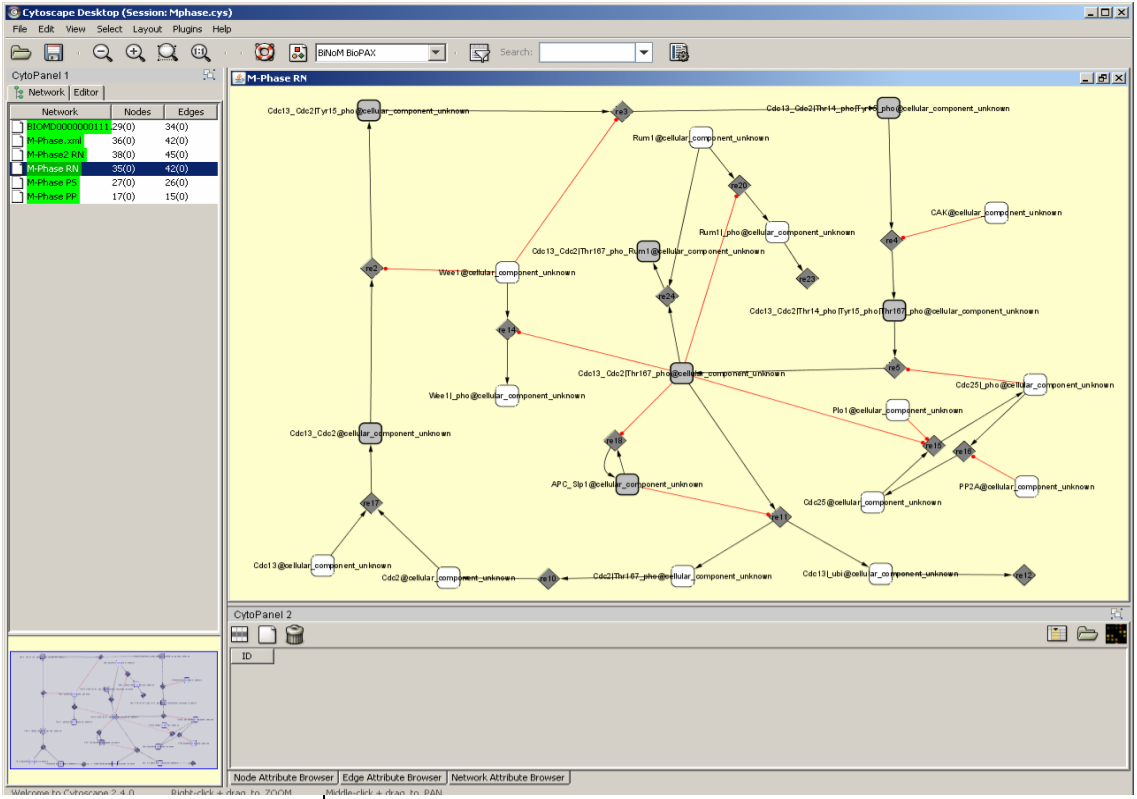
\includegraphics[width=0.8\textwidth]{graphics/View_BioPAX_of_Novak}
\caption{BioPAX view of Novak et al. model.}
\label{View_BioPAX_of_Novak}
\end{figure}
\begin{figure}
\centering
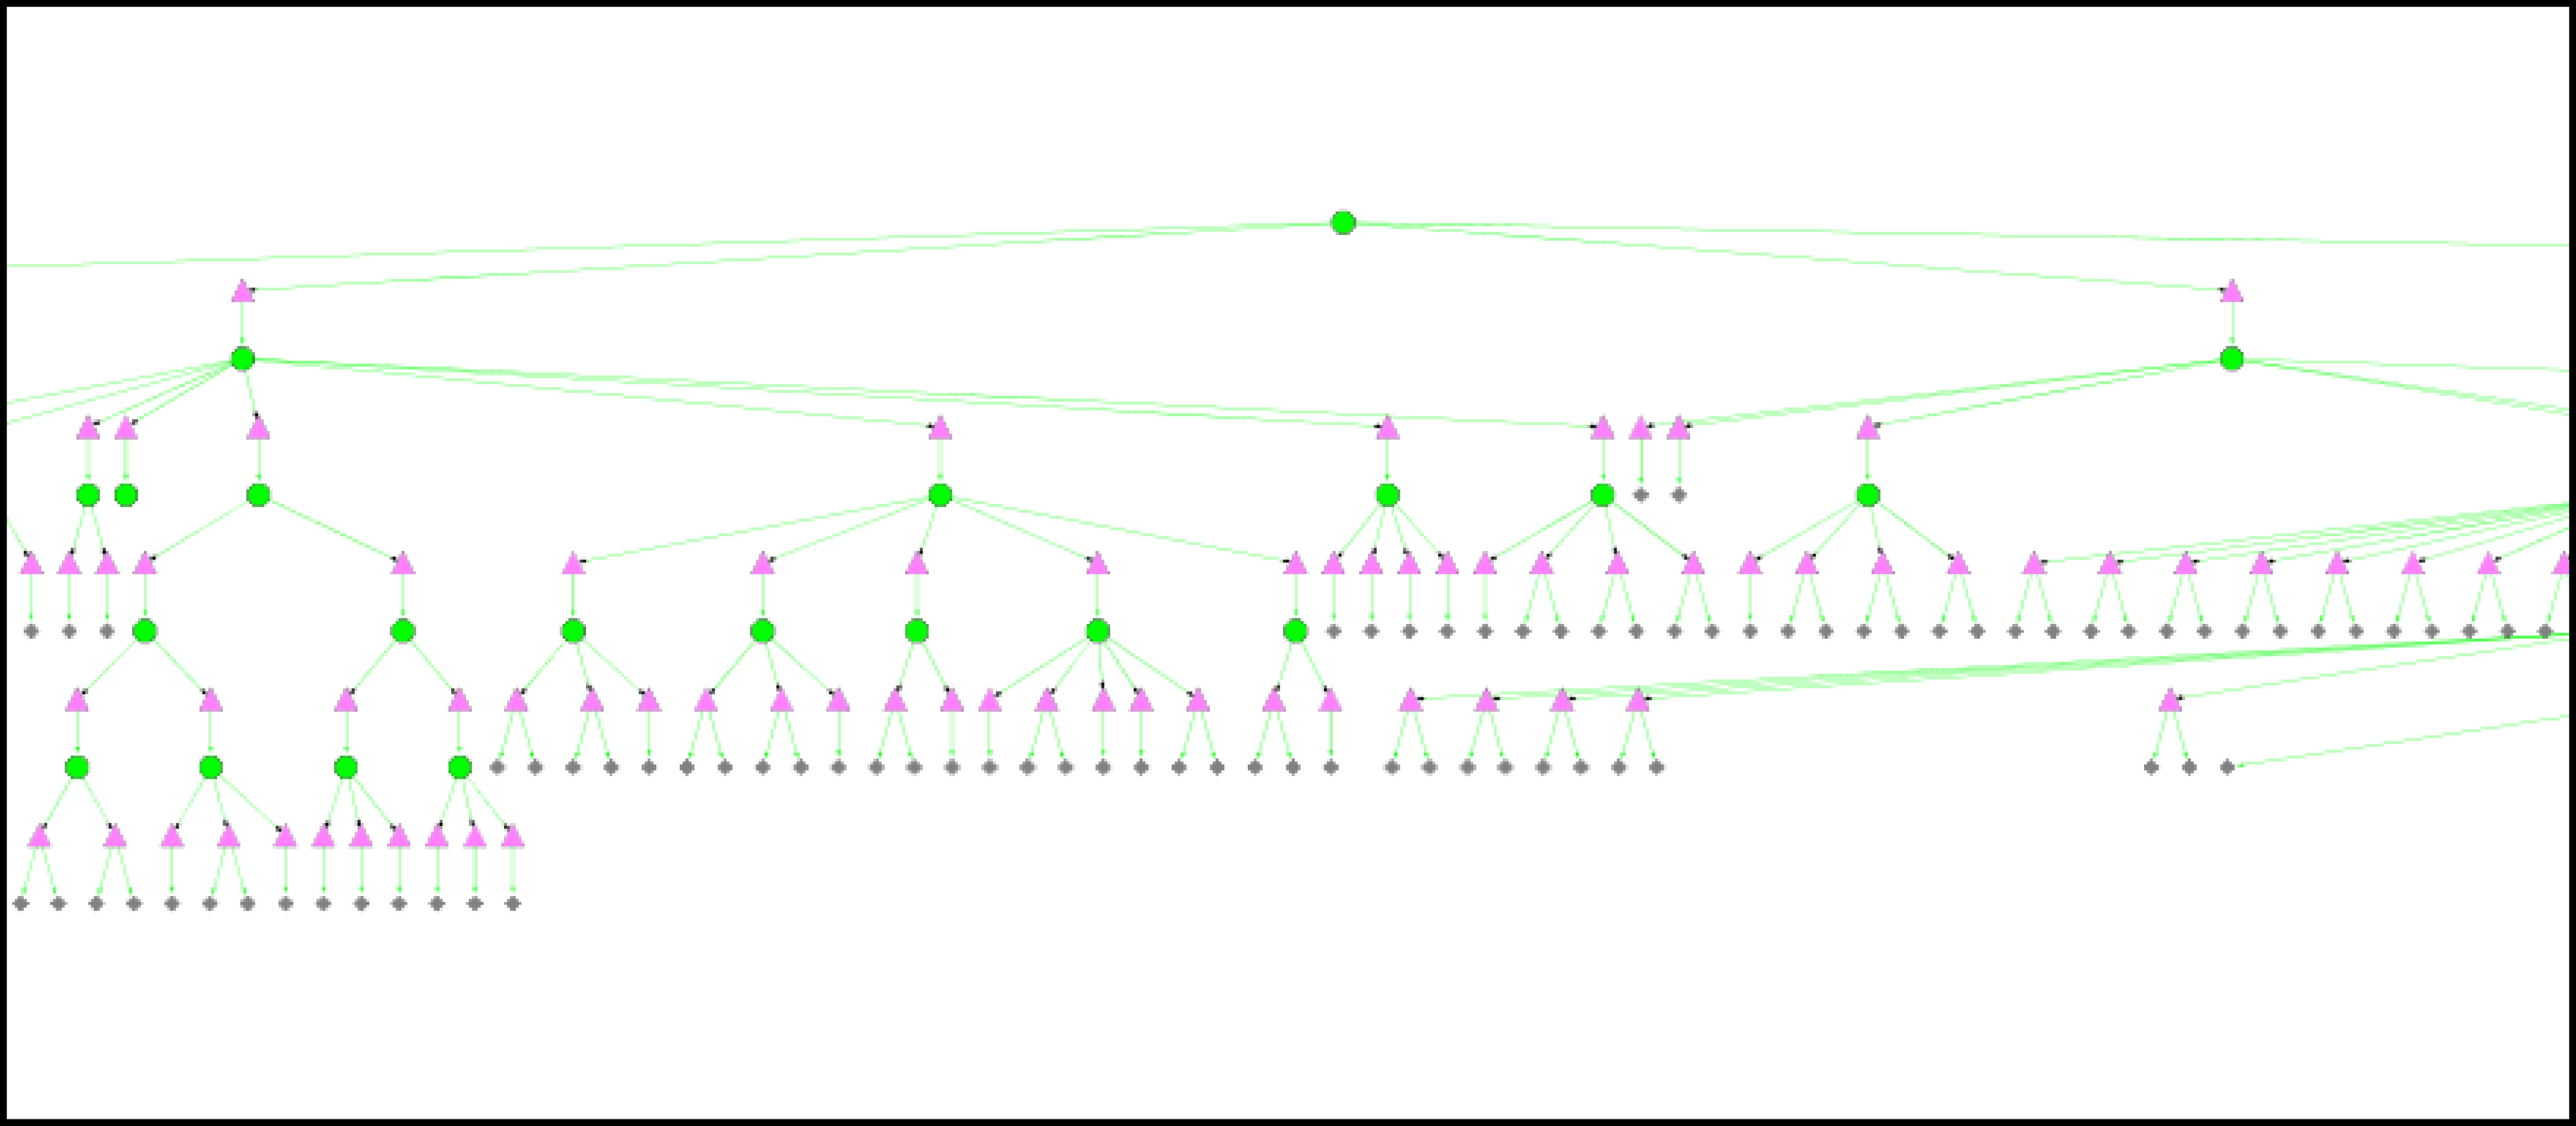
\includegraphics[width=0.8\textwidth]{graphics/Apoptosis_pathway_hierarchical_structure}
%\caption{Apoptosis pathway hierarchical structure. Green nodes represent pathways, pink triangular nodes represent steps, and grey nodes represent reactions. From the apoptosis node (top node in red), the cell can choose through 5 different paths. The red-colored path shows one of them, the activation of apoptosis via the intrinsic pathway, leading to the cleavage of caspases 3.}
\caption{Apoptosis pathway hierarchical structure. Green nodes represent
pathways, pink triangular nodes represent steps, and grey nodes represent
reactions.}
\label{Apoptosis_pathway_hierarchical_structure}
\end{figure}
\\In the case of creating the pathway structure interface, several choices are offered:
\begin{itemize}
\item Make Root Pathway Node: adds an extra node to which all pathways are connected. This feature can be useful for organizing the graph and joining separate and disjoint pathways.
\item Include Next Links: shows the ‘order’ of the reactions. From a node, an arrow indicates which node is the next step. This feature provides a timeline of the events in a pathway and could emphasize, for example, the linearity of a cascade.
\item Include Pathways: includes green nodes (figure~\ref{Apoptosis_pathway_hierarchical_structure}) which correspond to the names of the different pathways of the network.
\item Include interactions: shows explicitly the reactions involved in the pathway (lower grey nodes in figure~\ref{Apoptosis_pathway_hierarchical_structure}).
\end{itemize}\
\textbf{Plugins$\Rightarrow$BiNoM 2.1$\Rightarrow$BiNoM I/O$\Rightarrow$Import BioPAX 3 Document from URL}\\
A BioPAX 3 document can also be imported directly from a URL. The web address must be typed in the dialog window.



\subsection{Import CellDesigner document}
\textbf{Plugins$\Rightarrow$BiNoM 2.1$\Rightarrow$BiNoM I/O$\Rightarrow$Import CellDesigner Document from file}\\
The model can be drawn – or downloaded\cite{novak1998model} – in CellDesigner (figure~\ref{CellDesigner_view_of_yeast_cell_division}) and saved as M-Phase.xml.\\
The “Import CellDesigner Document from file” function imports a model from CellDesigner to Cytoscape.  A dialog window opens and M-Phase.xml needs to be selected and imported (figure~\ref{Cytoscape_view_of_yeast_cell_division}).\\
\begin{figure}
\centering
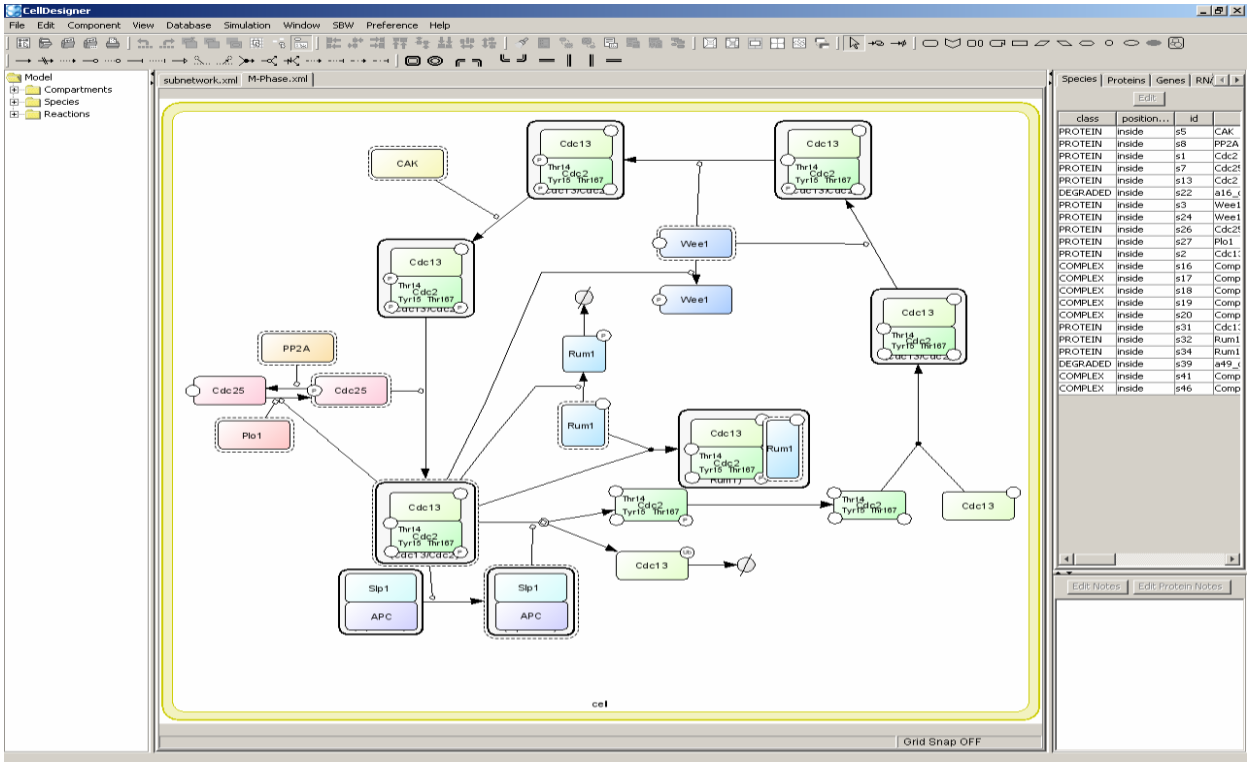
\includegraphics[width=0.8\textwidth]{graphics/CellDesigner_view_of_yeast_cell_division}
\caption{CellDesigner view of the cell division cycle model of fission yeast\cite{novak1998model}}
\label{CellDesigner_view_of_yeast_cell_division}
\end{figure}\begin{figure}
\centering
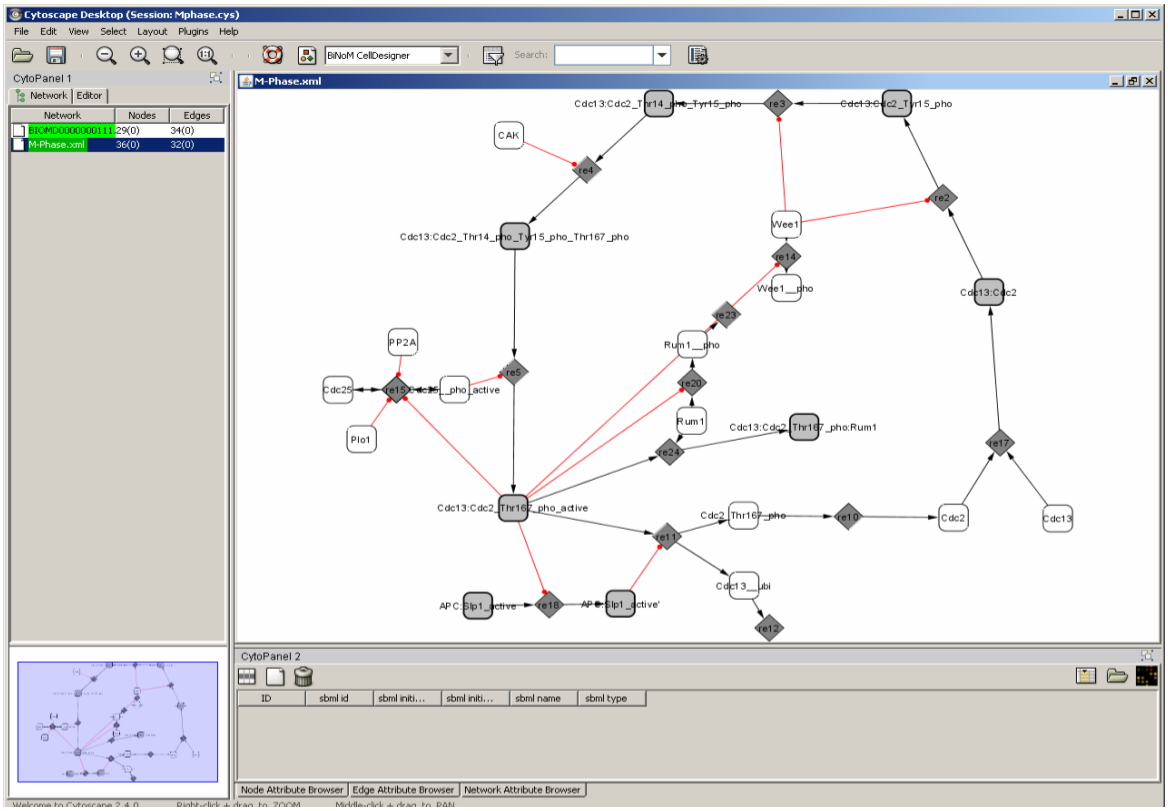
\includegraphics[width=0.8\textwidth]{graphics/Cytoscape_view_of_yeast_cell_division}
\caption{Cytoscape view of the cell division cycle model of fission yeast from a CellDesigner document}
\label{Cytoscape_view_of_yeast_cell_division}
\end{figure}
\\Figure~\ref{CellDesigner_view_of_yeast_cell_division}~and~\ref{Cytoscape_view_of_yeast_cell_division} show the same model viewed by CellDesigner and Cytoscape respectively. The layout information from CellDesigner is imported automatically into Cytoscape.\\\\
In species notes in CellDesigner “Attribute name:Value” as HUGO:E2F1 (without blank) is converted in Cytoscape as the attribute HUGO with the value E2F1 for the specie.\\\\



\subsection{Import CSML document}
\textbf{Plugins$\Rightarrow$BiNoM 2.1$\Rightarrow$BiNoM I/O$\Rightarrow$Import CSML document}\\
BiNoM imports a CSML (Cell System Markup Language, csml.org)



\subsection{Import influence network from AIN file} \label{Import_AIN_file}

\textbf{Plugins$\Rightarrow$BiNoM 2.1$\Rightarrow$BiNoM I/O$\Rightarrow$Import AIN file}\\

This option proposes to automatically import an influence network in Cytoscape
from a simple tab-delimited text file. We call the format of the
text file AIN (Annotated Influence Network). Basically each row of the text file is encoding an
interaction between two species, with a few optional descriptive fields. The precise
format for each field is described in the appendices (section~\ref{AIN_file_format}). 

The AIN file of the apoptosis model ExamplApop.txt is imported. First, the user
is asked to manage the families (groups of genes or proteins, see the appendices
for a precise description): they can be expanded (replacing the family by all
its members) or collapsed (replacing all family members by the name of the
family). See figure~\ref{AIN_dialog_for_families_management}.\\\\

\begin{figure}
\centering
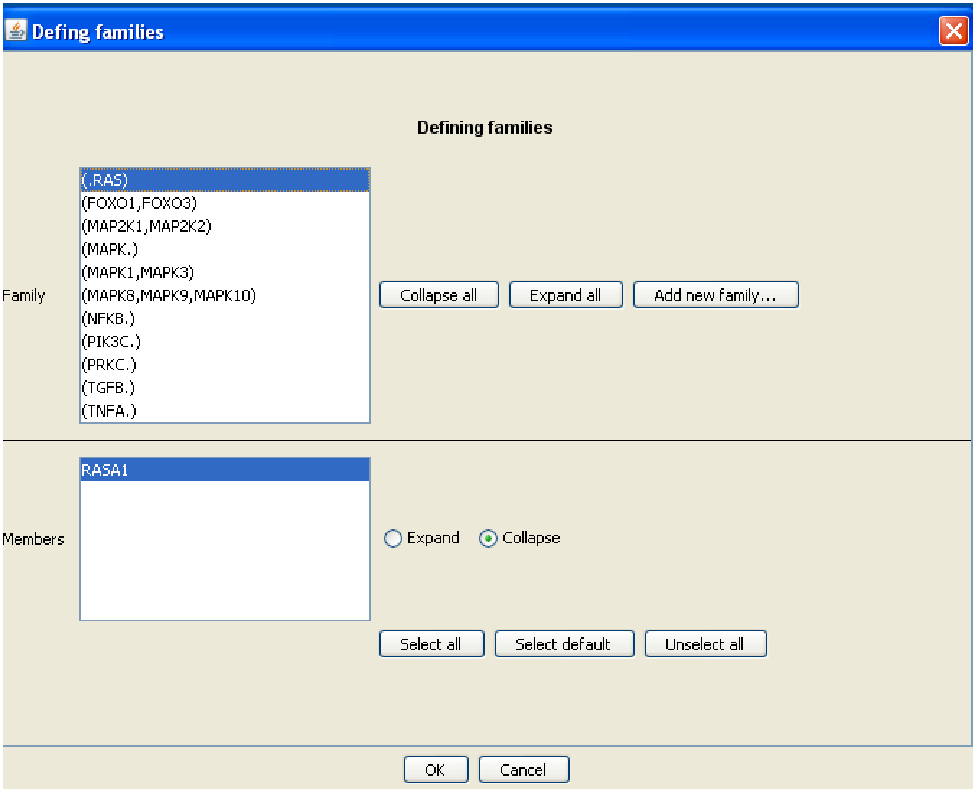
\includegraphics[width=0.8\textwidth]{graphics/AIN_dialog_for_families_management}
\caption{Dialog window for families management when importing the apoptosis network influence file (AIN format). BiNoM automatically detects gene families and proposes to either collapse or expand them.}
\label{AIN_dialog_for_families_management}
\end{figure}

Then a dialog window proposes to add constitutive reactions: influences that
link proteins (or families) to their complexes and proteins (or families) to
their phosphorylated state. See
figure~\ref{AIN_dialog_for_constitutive_reactions}.\\\\

\begin{figure}
\centering
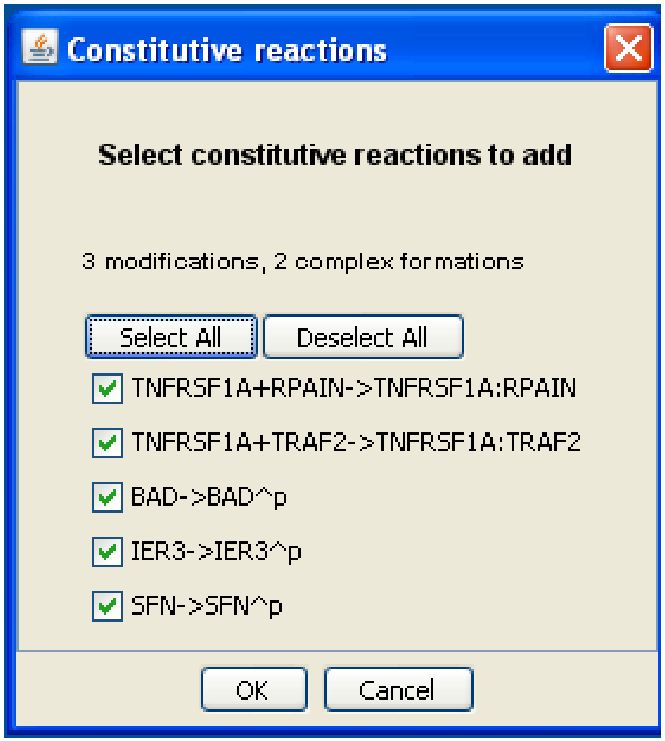
\includegraphics[width=0.5\textwidth]{graphics/AIN_dialog_for_constitutive_reactions}
\caption{Dialog window for constitutive reactions when importing apoptosis influence file. BiNoM detects all possible constitutive reactions and proposes to add them.}
\label{AIN_dialog_for_constitutive_reactions}
\end{figure}
The imported network is synchronized with BioPAX format that includes the annotations of the AIN file. All this information can be accessed via “BioPAX 3 property editor” (see BioPAX Utils, section ~\ref{BioPAX_Property_Editor}).



\subsection{Import reaction network from BiNoM reaction format file} \label{Import_reaction_format}
This function is available in the experimental version of BiNoM. 
A network can be written as a list of reactions. The network can be a biochemical reaction network or an influence network following the notation below.

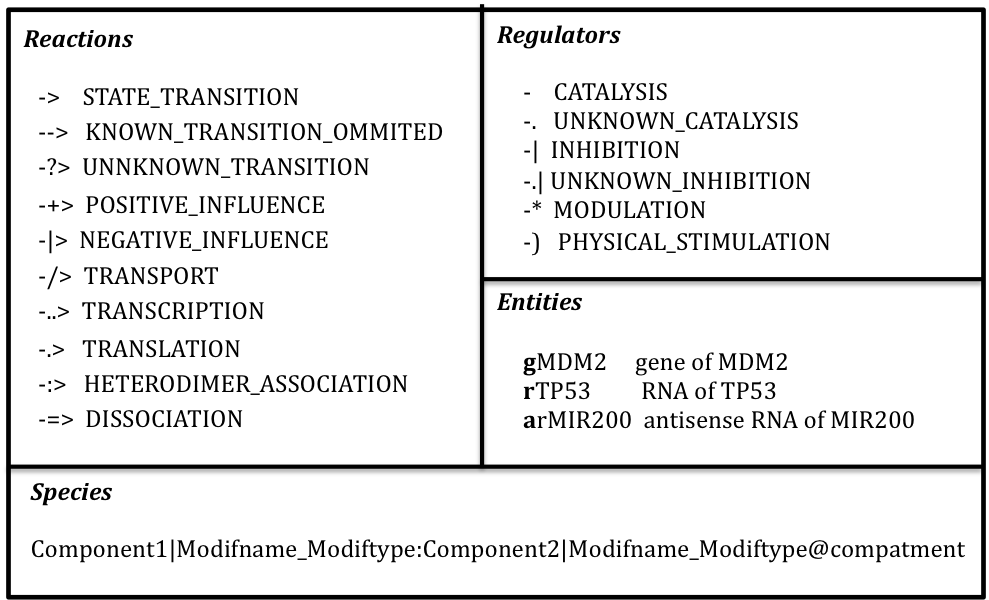
\includegraphics[width=1\textwidth]{graphics/syntax_text_network.png} 

Here we give an example of an influence network: 
\begin{verbatim}
MOMP-+>CYTOCHROME_C
APAF1-+>CASP9
SMAC-|>XIAP
FADD-+>CASP8
CASP8-+>CASP3
CASP8-+>BID
BAX-|>MOMP
CASP9-+>CAPS3
XIAP-|>CASP3
XIAP-|>CASP9
BID-+>MOMP
\end{verbatim}

The file must be saved in a txt format (with extension .txt). Here, the file is saved: apoptosis.txt

A network written with the BiNoM reaction format can then be imported in Cytoscape. \\
\textbf{Plugins$\Rightarrow$BiNoM 2.5$\Rightarrow$BiNoM I/O$\Rightarrow$Import reaction network from BiNoM reaction format file}\\

Choose apoptosis.txt

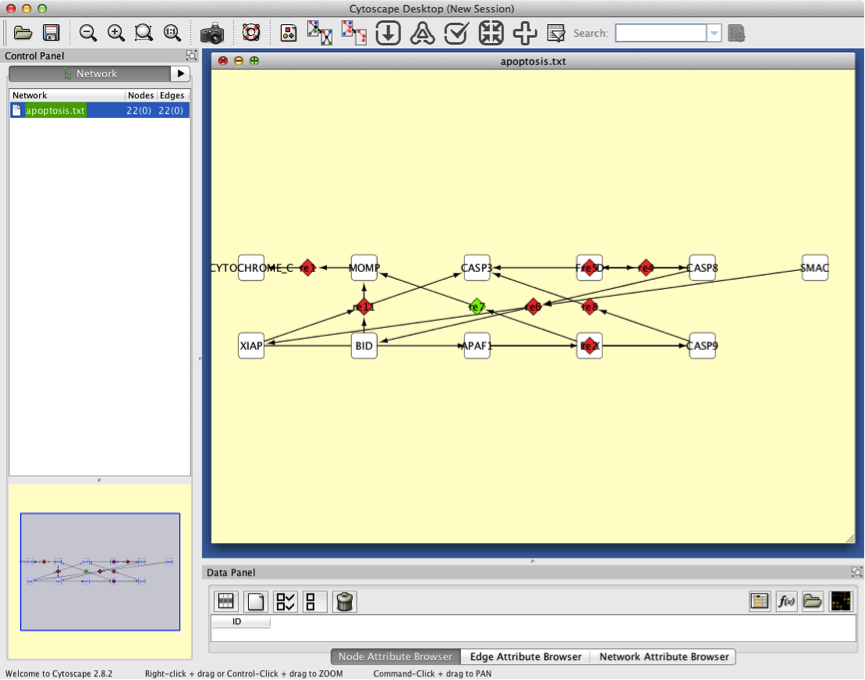
\includegraphics[width=1\textwidth]{graphics/Import_brff.png} 
% \caption{Network written with BiNoM format file and imported in Cytoscape. No layout is applied here.}



\subsection{Export current network to BioPAX 3 or to CellDesigner} \label{Export_current_network}
The Cytoscape networks can be exported in BioPAX and CellDesigner by:
\begin{itemize}
\item \textbf{Plugins$\Rightarrow$BiNoM 2.1$\Rightarrow$BiNoM I/O$\Rightarrow$Export current network to BioPAX 3}
\item \textbf{Plugins$\Rightarrow$BiNoM 2.1$\Rightarrow$BiNoM I/O$\Rightarrow$Export current network to CellDesigner}
\end{itemize}
\includegraphics[width=20pt,height=20pt]{graphics/warning} The network to be exported should be associated to an existing CellDesigner or BioPAX file by using the functions:
\begin{itemize}
\item Associate BioPAX Source, see section~\ref{Associate_BioPAX_Source}.
\item Associate CellDesigner Source,see~\ref{Associate_CellDesigner_Source}.
\end{itemize}
BiNoM is able to convert CellDesigner to BioPAX, and BioPAX
reaction network interface to pure SBML. BiNoM can also export only a
part of a CellDesigner and BioPAX file, visible in the current Cytoscape network
(interface). During the export operation, BiNoM can merge a part of
associated BioPAX file with another part that has been saved already. BiNoM can modify the
content of a BioPAX file. \\\\

\includegraphics[width=20pt,height=20pt]{graphics/warning} BiNoM is NOT able to
create a CellDesigner file with all the graphical notations from a BioPAX file or from
scratch, and it is also not able to modify the content of a CellDesigner file.\\\\

Here are a couple of typical scenarios where BiNoM export operations can be useful.
\begin{enumerate}
\item User imports a big BioPAX file as reaction network and using Cytoscape creates a new subnetwork from the global reaction graph. After he can export this subnetwork into a separate self-containing BioPAX file.
\item User imports the pathway structure of a big BioPAX file and selects only a few pathway or pathwayStep nodes he is interested in. After he can export a part of the BioPAX file necessary to define these pathways.
\item User imports a BioPAX file as reaction network, selects a subnetwork and exports it as pure SBML to be used for creation of a computational model of this subpart later.
\item User imports CellDesigner file, selects a subnetwork and exports it as a CellDesigner file: it can be useful for creating a CellDesigner image of a network module of a big reaction network.
\item User imports CellDesigner file, selects a subnetwork and exports it as a BioPAX file (some SBML-specific information such as parameters values will be lost).
\end{enumerate}
The networks created as a result of the import operation are already associated to the corresponding BioPAX or CellDesigner files. However, if the XGMML file is saved and used in another Cytoscape session, or if a new network is created from the initial network with Cytoscape New menu then this association is lost.\\\\
To perform export operation, the network should be Re-associated to the corresponding file (from which it is originated) through Plugins$\Rightarrow$BiNoM 2.1$\Rightarrow$BiNoM I/O$\Rightarrow$Associate$\ldots$ operation. For huge BioPAX files the association might take some time for the first association, but once the file is loaded into memory cache, the following associations are almost instantaneous.\\\\
To understand better what BiNoM can do or can not, read the sections \ref{Attributed_graph_model}, \ref{BiNoM_Naming_Service} and \ref{Standard_BioPAX_Interfaces} about the BiNoM data model.



\subsection{Create CellDesigner file from current network}
This function is available in the experimental version of BiNoM. \\
\textbf{Plugins$\Rightarrow$BiNoM 2.5$\Rightarrow$BiNoM I/O$\Rightarrow$Create CellDesigner file from current network}\\

The file needs to be saved with the extension .xml.

This function is different than:\\
\textbf{Plugins$\Rightarrow$BiNoM 2.5$\Rightarrow$BiNoM I/O$\Rightarrow$Export current network to CellDesigner}\\
With the export function, the user needs to associate the network to an existing CellDesigner file. It is useful when creating a subnetwork from an existing Celldesigner network, for instance.

Here we save our network to apoptosis.xml.

Open the saved file into CellDesigner. Apply the orthogonal layout or re-arrange the network as you wish.


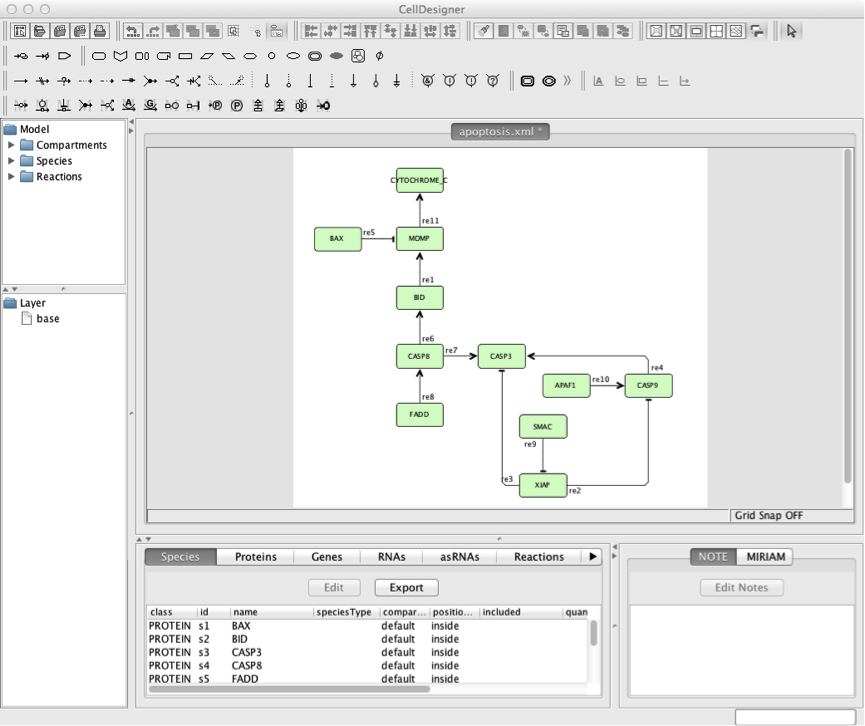
\includegraphics{graphics/Import_CD_brff.png} 
%\caption{Network written with BiNoM format file and imported in CellDesigner. Orthogonal layout is applied here.}

The network exported in CellDesigner can also be a network imported from a BioPAX file. This function allows the visualization of a BioPAX file in CellDesigner.  For that, you need to import a BioPAX file using the function:\\
\textbf{Plugins$\Rightarrow$BiNoM 2.5$\Rightarrow$BiNoM I/O$\Rightarrow$Import reaction network from BioPAX}\\

Choose exampleBIOPAX.owl.

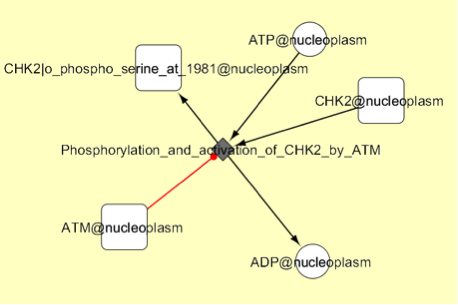
\includegraphics{graphics/example_BioPAX.png} 

Then, export the current network to CellDesigner using the function:\\
\textbf{Plugins$\Rightarrow$BiNoM 2.5$\Rightarrow$BiNoM I/O$\Rightarrow$Create CellDesigner file from current network}\\

Save the file as: example.BIOPAX.xml

Open the file in CellDesigner:\\

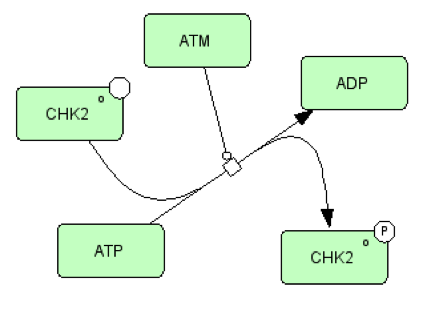
\includegraphics{graphics/BioPAX_to_CD.png} 



\subsection{Export current network to SBML}
\textbf{Plugins$\Rightarrow$BiNoM 2.1$\Rightarrow$BiNoM I/O$\Rightarrow$Export current network to SBML}\\
Export the current network to pure SBML level 2.


\subsection{Export network to BiNoM reaction format}
\textbf{Plugins$\Rightarrow$BiNoM 2.1$\Rightarrow$BiNoM I/O$\Rightarrow$Export network to BiNoM reaction format}\\

This function allows to translate a network into a list of reactions. The file is saved as a text file.

As an example, we imported the file M-Phase.xml and exported the network to BiNoM reaction format file. The file is saved as a txt file (MPhasebrff.txt) as follows: 

\begin{verbatim}
(APC':Slp1')||active'|active
(APC:Slp1)||active
Cdc13:Cdc2|Thr167_pho:Rum1
Rum1|pho
Rum1
Cdc13|ubi
(Cdc13:Cdc2|Thr167_pho)||active
Cdc13:Cdc2|Thr14_pho|Tyr15_pho|Thr167_pho
Cdc13:Cdc2|Thr14_pho|Tyr15_pho
Cdc13:Cdc2|Tyr15_pho
Cdc13:Cdc2
Cdc13
Plo1
Cdc25|pho|active
Wee1|pho
Wee1
Cdc2|Thr167_pho
Cdc25
Cdc2
PP2A
CAK

Rum1+(Cdc13:Cdc2|Thr167_pho)||active-:>Cdc13:Cdc2|Thr167_pho:Rum1
Rum1|pho->null
Rum1-(Cdc13:Cdc2|Thr167_pho)||active->Rum1|pho
(APC:Slp1)||active-(Cdc13:Cdc2|Thr167_pho)||active->(APC':Slp1')||active'|active
Cdc13+Cdc2-:>Cdc13:Cdc2
Cdc25|pho|active-PP2A->Cdc25
Cdc25-(Cdc13:Cdc2|Thr167_pho)||active-Plo1->Cdc25|pho|active
Wee1-(Cdc13:Cdc2|Thr167_pho)||active->Wee1|pho
Cdc13|ubi->null
(Cdc13:Cdc2|Thr167_pho)||active-(APC':Slp1')||active'|active-=>Cdc13|ubi+Cdc2|Thr167_pho
Cdc2|Thr167_pho->Cdc2
Cdc13:Cdc2|Thr14_pho|Tyr15_pho|Thr167_pho-Cdc25|pho|active->(Cdc13:Cdc2|Thr167_pho)||active
Cdc13:Cdc2|Thr14_pho|Tyr15_pho-CAK->Cdc13:Cdc2|Thr14_pho|Tyr15_pho|Thr167_pho
Cdc13:Cdc2|Tyr15_pho-Wee1->Cdc13:Cdc2|Thr14_pho|Tyr15_pho
Cdc13:Cdc2-Wee1->Cdc13:Cdc2|Tyr15_pho
\end{verbatim}

Note that BiNoM lists first all the species and then the reactions. 


We propose three scenarios that use BiNoM reaction format file.
\begin{itemize}
\item First scenario: create a CellDesigner file from a textual model
	\begin{enumerate}
		\item Write network in text format:
			\begin{verbatim}
			A => B
			B+C=>D+E
			...
			\end{verbatim}
		\item Import reaction network in Cytoscape using BiNoM
		\item Create CellDesigner file from current network
		\item Open CellDesigner and import the newly saved file
	\end{enumerate}
\item Second scenario: create a CellDesigner file from BioPAX file
	\begin{enumerate}
		\item Import a BioPAX file in Cytoscape
		\item Create CellDesigner file from current network
		\item Open CellDesigner and import the newly saved file
	\end{enumerate}
\end{itemize}


\subsection{Associate BioPAX 3 Source} \label{Associate_BioPAX_Source}
\textbf{Plugins$\Rightarrow$BiNoM 2.1$\Rightarrow$BiNoM I/O$\Rightarrow$Associate BioPAX 3 Source}\\
Associate a BioPAX 3 Source to allow exportation in BioPAX 3 as explained in section~\ref{Export_current_network}




\subsection{Save whole associated BioPAX 3 as}
When the content of the BioPAX file is modified (through the BioPAX property editor, see section ~\ref{BioPAX_Property_Editor}), it can be saved as a whole (not only the visible part) by\\
\textbf{Plugins$\Rightarrow$BiNoM 2.1$\Rightarrow$BiNoM I/O$\Rightarrow$Save whole associated BioPAX 3 as}\\
Otherwise, all modifications made in the different interfaces are lost. Changes are visible but only recorded permanently when the document is saved to a file.



\subsection{Associate CellDesigner Source}\label{Associate_CellDesigner_Source}
\textbf{Plugins$\Rightarrow$BiNoM 2.1$\Rightarrow$BiNoM I/O$\Rightarrow$Associate BioPAX 3 Source} \\
Associate a CellDesigner Source to allow exportation in CellDesigner as explained in section~\ref{Export_current_network}



\subsection{List all reactions}
\textbf{Plugins$\Rightarrow$BiNoM 2.1$\Rightarrow$BiNoM I/O$\Rightarrow$List all reactions} \\
Display list of reactions, can be copied by control+A then control+C.



\subsection{List all nodes}
\textbf{Plugins$\Rightarrow$BiNoM 2.1$\Rightarrow$BiNoM I/O$\Rightarrow$List all nodes} \\
Display list of nodes, can be copied by control+A then control+C.



\subsection{Color CellDesigner proteins}
\textbf{Plugins$\Rightarrow$BiNoM 2.1$\Rightarrow$BiNoM I/O$\Rightarrow$Color CellDesigner proteins}\\
Cytoscape allows coloring nodes according to values of attributes (for example expression data) by the powerful possibilities of VizMapper. The export to CellDesigner keeps the colors. This process can be used to color species in CellDesigner. The function Color CellDesigner proteins allows to color proteins in CellDesigner which describe the components of complexes.\\\\
The gene expression file is based on Hugo names, data in columns (first line title and tabulation as column separator):\\Hugo names\textless Tab\textgreater expression level 1\textless Tab\textgreater expression level 2$\ldots$\\\\
Open dialog box “Color CellDesigner proteins…”, input CellDesigner file name and gene expression file, click on ok. BiNoM generate a file *.conv where Hugo names are converted in protein names (links by annotation in CellDesigner, check if correct) and a CellDesigner file by column. When there are several Hugo name the highest is kept.\\\\
Figure~\ref{Colored_CellDesigner_view_by_ficticious_data} shows the aspect of colored proteins inside complexes.
\begin{figure}
\centering
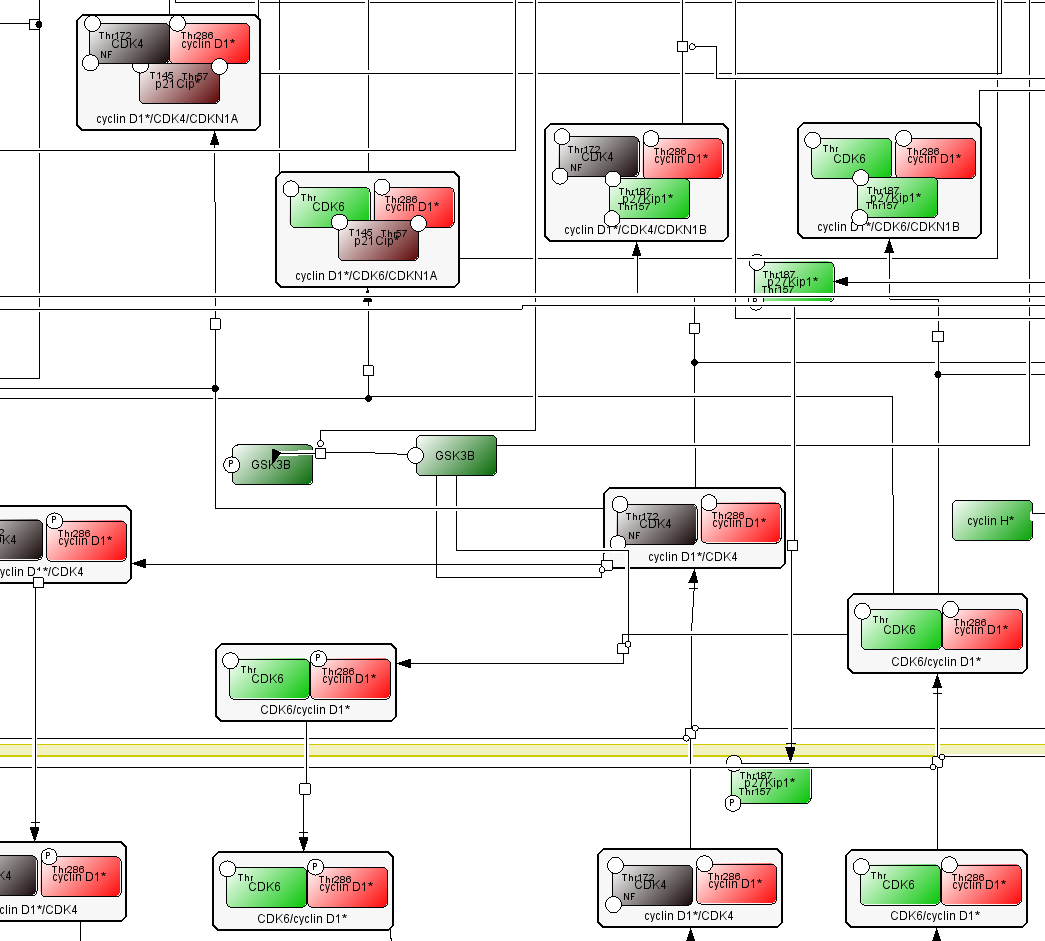
\includegraphics[width=0.8\textwidth]{graphics/Colored_CellDesigner_view_by_ficticious_data}
\caption{CellDesigner view of an extract from Rb-E2F\cite{calzone2008comprehensive} pathway colored by ficticious expression data}
\label{Colored_CellDesigner_view_by_ficticious_data}
\end{figure}



\subsection{Modify CellDesigner notes}
\textbf{Plugins$\Rightarrow$BiNoM 2.1$\Rightarrow$BiNoM I/O$\Rightarrow$Color CellDesigner proteins}\\
Modify in Cytoscape the notes of CellDesigner file when exporting.

\clearpage
\section{BiNoM Analysis}
We illustrate, here, the different functions of BiNoM related to the structural analysis, using the modified version of the Novak et al. model, M-Phase.xml as an example (figure~\ref{Cytoscape_view_of_the_M-Phase_network}).
\begin{figure}
\centering
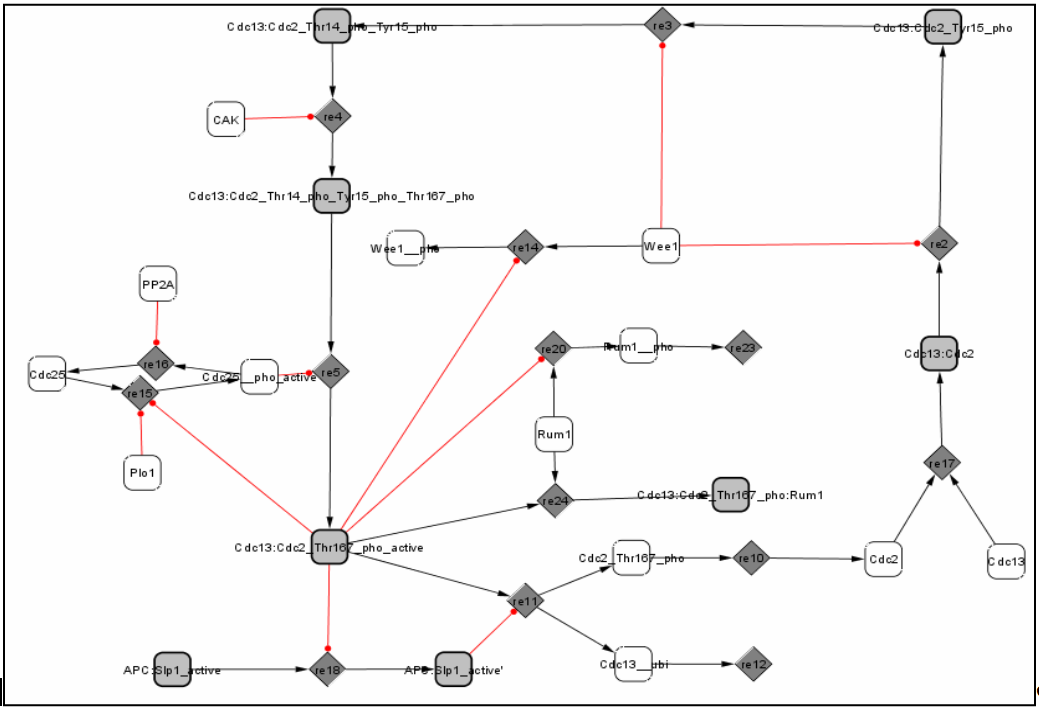
\includegraphics[width=0.8\textwidth]{graphics/Cytoscape_view_of_the_M-Phase_network.png}
\caption{Cytoscape view of the M-Phase network}
\label{Cytoscape_view_of_the_M-Phase_network}
\end{figure}
\\From the menu Plugins$\Rightarrow$BiNoM 2.1$\Rightarrow$ BiNoM analysis, we review all the functions one by one.

\subsection{Get connected components}
\textbf{Plugins$\Rightarrow$BiNoM 2.1$\Rightarrow$BiNoM Analysis$\Rightarrow$Get connected components}\\
This command dissociates the unconnected subparts of the network. In our case, since the network is already completely connected, the one obtained when choosing this function is the same as the initial one (called M-Phase.xml\_cc1).
\subsection{Get strongly connected components}
Plugins$\Rightarrow$BiNoM 2.1$\Rightarrow$BiNoM Analysis$\Rightarrow$Get strongly connected components\\
\begin{figure}
\centering
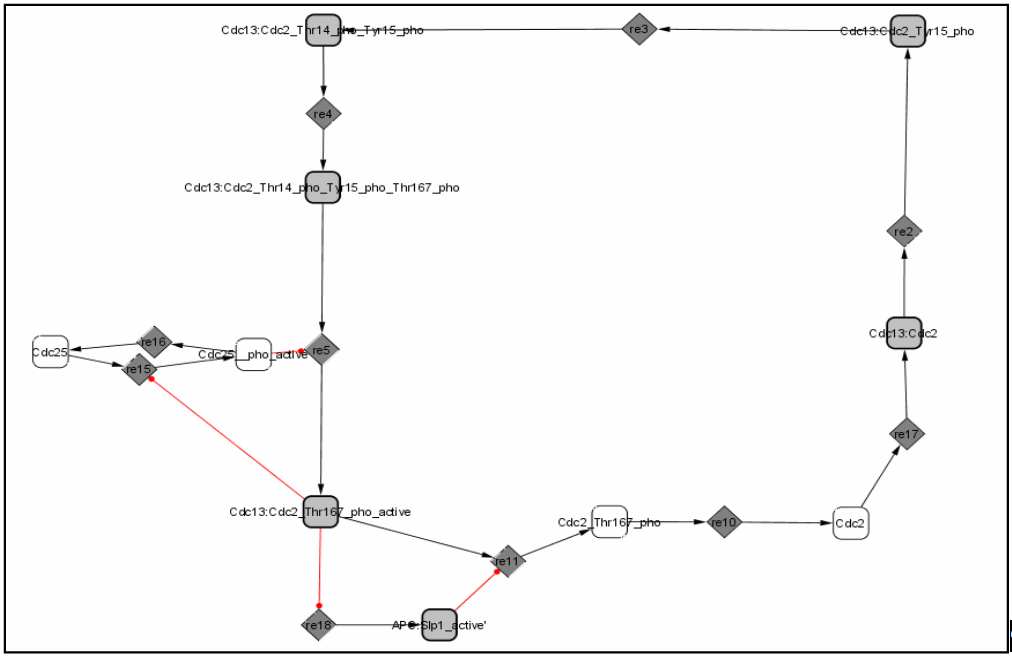
\includegraphics[width=0.8\textwidth]{graphics/Strongly_Connected_Component_of_M-Phase_network.png}
\caption{Strongly Connected Component of M-Phase network}
\label{Strongly_Connected_Component_of M-Phase_network}
\end{figure}
\\Based on Tarjan’s algorithm\cite{tarjan1972depth}, the strongly connected components are isolated. In simple words, the obtained network, M-Phase.xml\_scc1(figure~\ref{Strongly_Connected_Component_of M-Phase_network}), insures that there exists a path from one node to another and deletes the components which do not respond to this requirement.

\subsection{Prune Graph}
\textbf{Plugins$\Rightarrow$BiNoM 2.1$\Rightarrow$BiNoM Analysis$\Rightarrow$Prune graph}\\
Pruning the graph is equivalent to separating the network into three parts(figure~\ref{Prune_the_graph}: what comes in (M-Phase.xml\_in), what goes out (M-Phase.xml\_out) and the central cyclic part (M-Phase.xml\_scc).
\\This decomposition corresponds to the idea of the bow-tie structure developed by Broder and colleagues\cite{broder2000graph}. In our example, the central cyclic part is the same as figure~\ref{Strongly_Connected_Component_of M-Phase_network}, the strongly connected component. In other cases, it can be composed from several strongly connected components, connected or disconnected.\\
The Prune graph operation decomposes the current network into three parts: IN, OUT and SCC (the later can contain several strongly connected components).
\begin{figure}
\centering
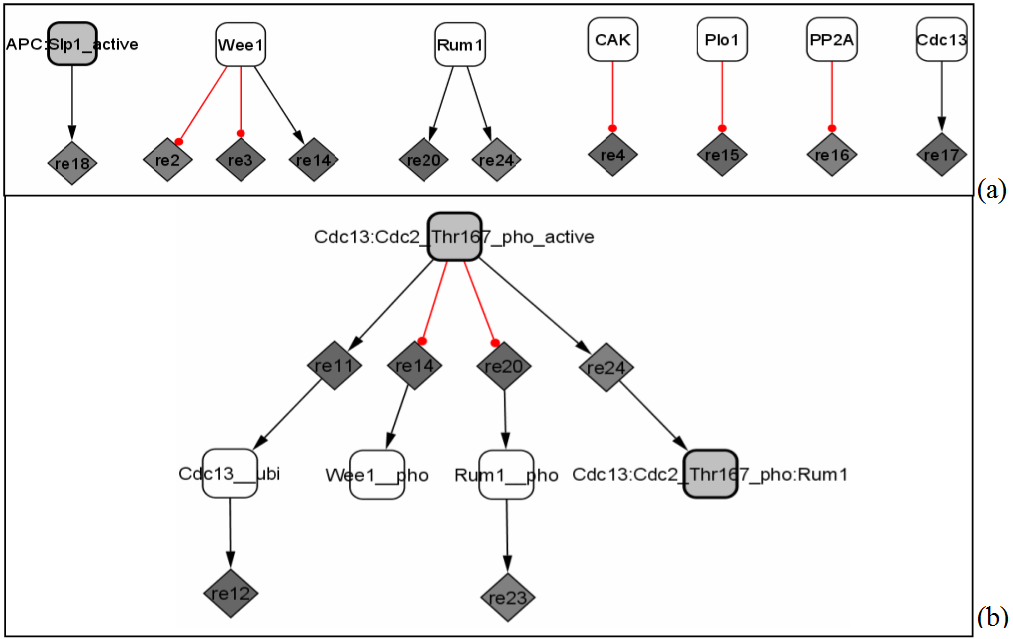
\includegraphics[width=0.8\textwidth]{graphics/Prune_the_graph}
\caption{Prune the graph. (a) Incoming flux: molecules involved in the IN part of the network, and (b) Outgoing flux: molecules involved in the OUT part of the network.}
\label{Prune_the_graph}
\end{figure}

\subsection{Get Material Components}
\textbf{Plugins$\Rightarrow$BiNoM 2.1$\Rightarrow$BiNoM Analysis$\Rightarrow$Get material components}\\
This function uses node name semantics to isolate sub-networks in which each protein takes part. In our example(figure~\ref{Material_Components}), seven sub-networks are created: M-Phase.xml\_Cdc13, M-Phase.xml\_Cdc2, M-Phase.xml\_Rum1, M-Phase.xml\_APC, M-Phase.xml\_Slp1, M-Phase.xml\_Cdc25 and M-Phase.xml\_Wee1. Some major overlaps between sub-networks are expected, as it is the case for Cdc2 and Cdc13 which form a complex.\\
\begin{figure}
\centering
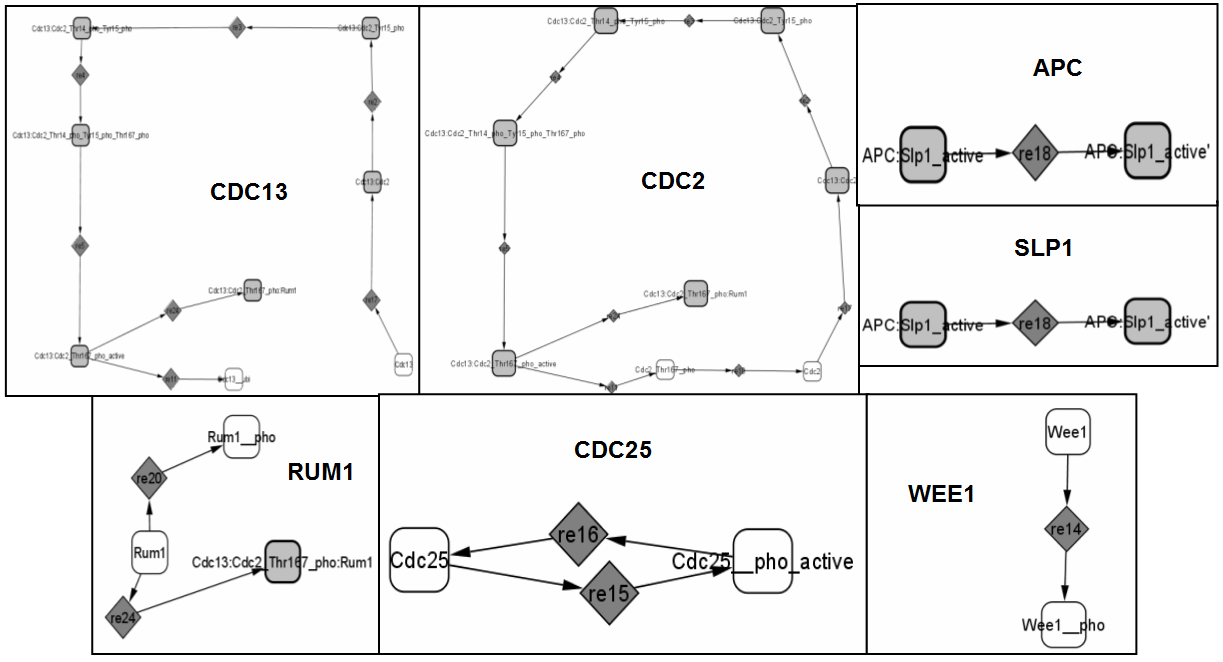
\includegraphics[width=0.8\textwidth]{graphics/Material_components}
\caption{Material Components}
\label{Material_Components}
\end{figure}

\subsection{Get Cycle Decomposition}
\textbf{Plugins$\Rightarrow$BiNoM 2.1$\Rightarrow$BiNoM Analysis$\Rightarrow$Get cycle decomposition}\\
This command decomposes the network into relevant directed cycles\cite{gleiss2001relevant}, using a modification of the Vismara’s algorithm\cite{vismara1997union}. Often, this feature gives information about the life cycle of a protein or a complex, about the feedbacks of the studied network, etc(figure~\ref{Minimal_cycle_decomposition_of_the M-Phase}). Note that the union of all the cycles corresponds to the strongly connected component figure~\ref{Strongly_Connected_Component_of M-Phase_network}.\\
\includegraphics[width=20pt,height=20pt]{graphics/warning} This operation can produce enormous number of cycles! Therefore it is rather suitable for analysis of small to moderate size networks. For a big network, one can start to understand the cyclic network structure by eliminating first the network hubs, which are contained in many network cycles. After that, the local, relatively short, cycles can be represented as meta-nodes (modules) and the analysis for cycles can be repeated.\\
\begin{figure}
\centering
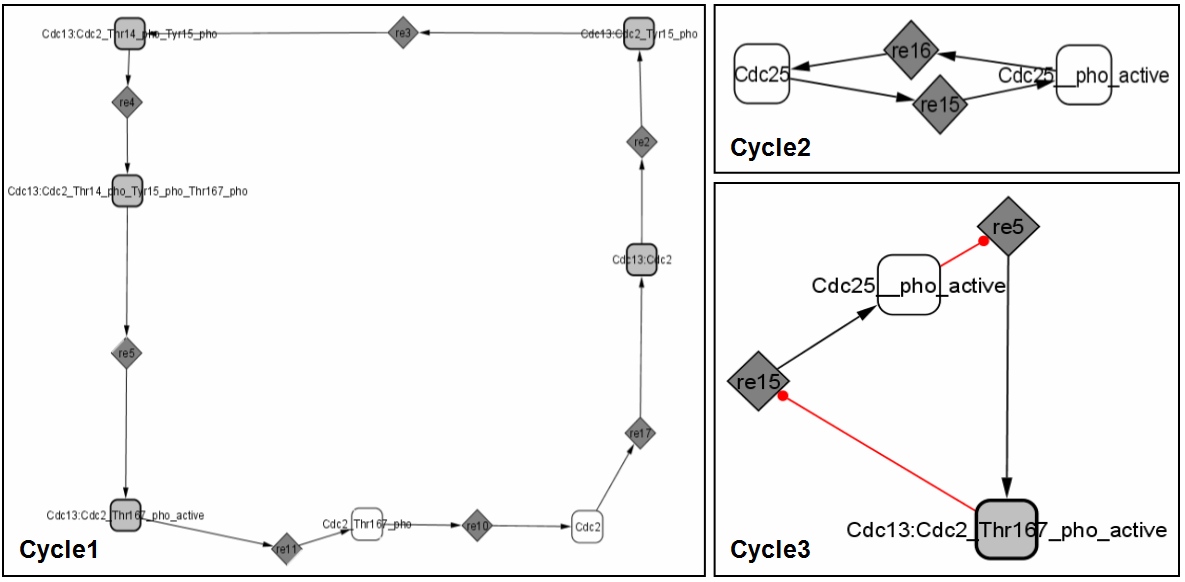
\includegraphics[width=0.8\textwidth]{graphics/Minimal_cycle_decomposition_of_the_M-Phase}
\caption{Minimal cycle decomposition of the M-Phase network.  Cycle 1 includes CDC2 and CDC13 proteins, Cycle 2 CDC25 and Cycle 3 shows the feedback existing between CDC13/CDC2 and CDC25.}
\label{Minimal_cycle_decomposition_of_the M-Phase}
\end{figure}

\subsection{Path Analysis}\label{Path_Analysis}
\textbf{Plugins$\Rightarrow$BiNoM 2.1$\Rightarrow$BiNoM Analysis$\Rightarrow$Path analysis}\\
In a network, it can become handy to find out if there exists a path (or paths) from one species to another, or to verify that a protein or a protein complex is reachable from a starting molecule(figure~\ref{Path_Analysis_All_the_paths}). Provided (an) initial source and target protein(s) that are selected first on the graph then in the dialog window, the command Path analysis can find: the shortest paths, the optimal and suboptimal shortest paths, or all the non-intersecting paths (does not include inner loops), using a finite number of intermediary nodes (use finite breadth search radius), for either directed or undirected paths (figure~\ref{Path_Analysis_Pop-up_window}).\\
\includegraphics[width=20pt,height=20pt]{graphics/warning} In big networks the number of paths can be exponential! It is recommended to find the shortest path first, take its length and increment gradually the breadth search radius starting from this value to find the second shortest, third shortest, etc., paths.\\
\begin{figure}
\centering
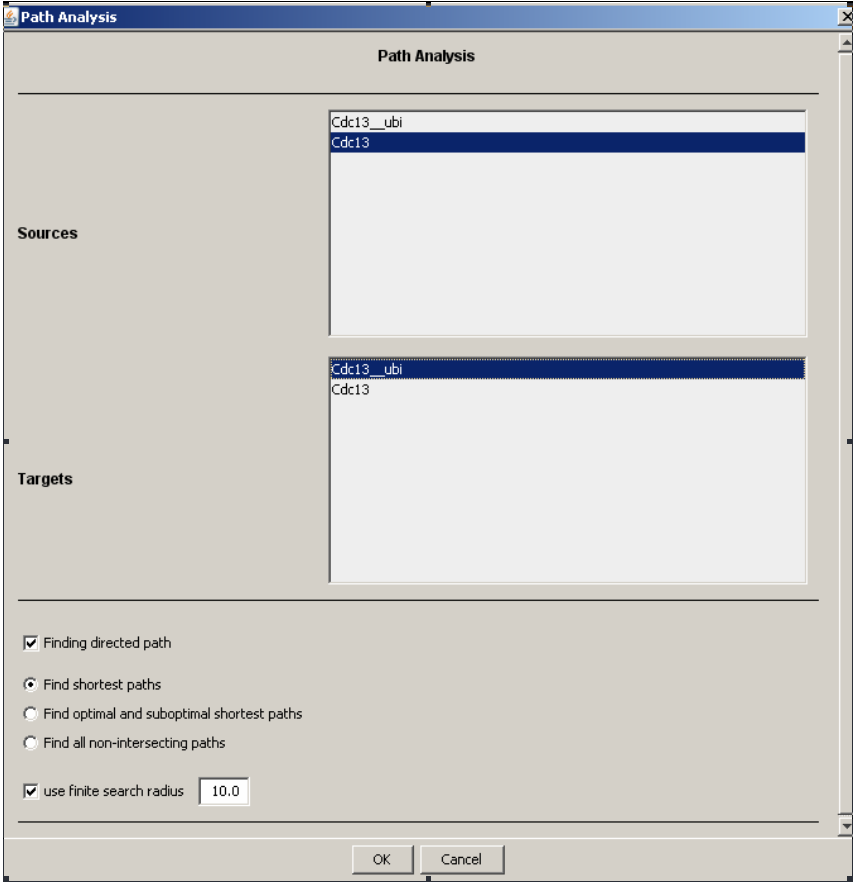
\includegraphics[width=0.8\textwidth]{graphics/Path_Analysis_Pop-up_window}
\caption{BiNoM Path Analysis: Pop-up window in which the source(s) and the target(s) need to be specified along with the type of paths (shortest, optimal shortest or all paths).}
\label{Path_Analysis_Pop-up_window}
\end{figure}
\begin{figure}
\centering
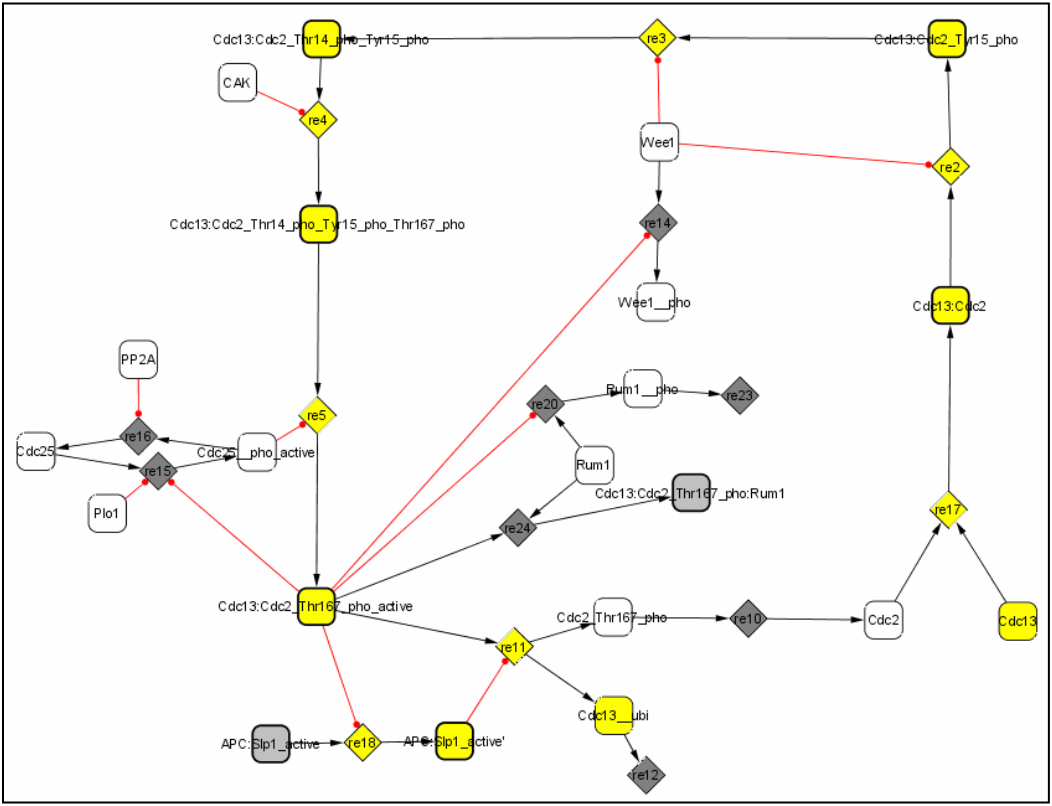
\includegraphics[width=0.8\textwidth]{graphics/Path_Analysis_All_the_paths}
\caption{Path Analysis: All the paths leading from one molecular species (Cdc13) to another (Cdc13\_ubi, ubiquitinated form of Cdc13) are highlighted in yellow.}
\label{Path_Analysis_All_the_paths}
\end{figure}

\subsection{Extract subnetwork}
\textbf{Plugins$\Rightarrow$BiNoM 2.1$\Rightarrow$BiNoM Analysis$\Rightarrow$Extract subnetwork}\\
Extract a subnetwork from selected nodes of a network with various options (figure~\ref{Extract_subnetwork_dialog}).
\begin{figure}
\centering
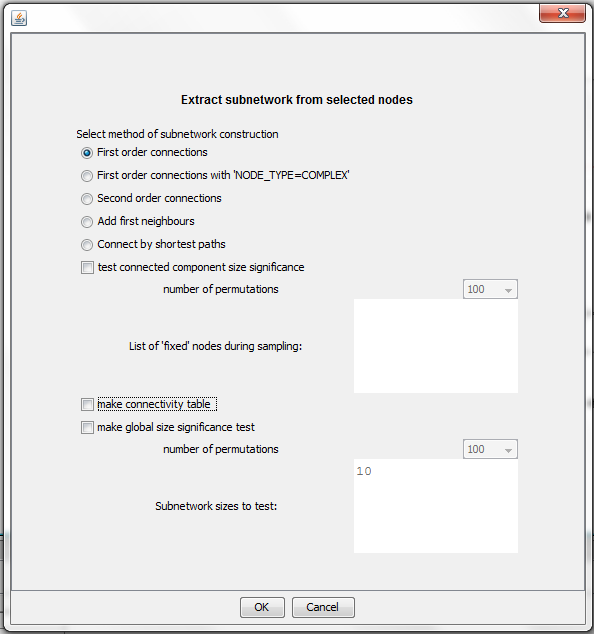
\includegraphics[width=0.8\textwidth]{graphics/Extract_subnetwork_dialog}
\caption{Dialog of the ``Extract subnetwork'' function showing the different options available.}
\label{Extract_subnetwork_dialog}
\end{figure}

\subsection{Calc centrality, Inbetweenness undirected, Inbetweenness directed}
\textbf{Plugins$\Rightarrow$BiNoM 2.1$\Rightarrow$BiNoM Analysis$\Rightarrow$Calc centrality$\Rightarrow$Inbetweenness undirected}
\textbf{Plugins$\Rightarrow$BiNoM 2.1$\Rightarrow$BiNoM Analysis$\Rightarrow$Calc centrality$\Rightarrow$Inbetweenness directed}
Display centrality of nodes in cases undirected and directed.

%\subsection{Generate Modular View}
%\textbf{Plugins$\Rightarrow$BiNoM$\Rightarrow$analysis$\Rightarrow$Generate modular view}\\
%Given the initial diagram and some modules (which could be sub-networks of the initial network), it is possible to reconstruct a modular view of the network. For our example, we choose the initial network to be M-Phase.xml and the subparts or modules, the seven sub-networks corresponding to the material components described in (4). From these seven sub-networks only six are selected since two of them, Slp1 and APC, are exactly the same.\\
%The sub-networks or modules need to be specified in the “creating modular view” window (figure~\ref{Modular_view_Pop-up_window}).\\
%\begin{figure}
%\centering
%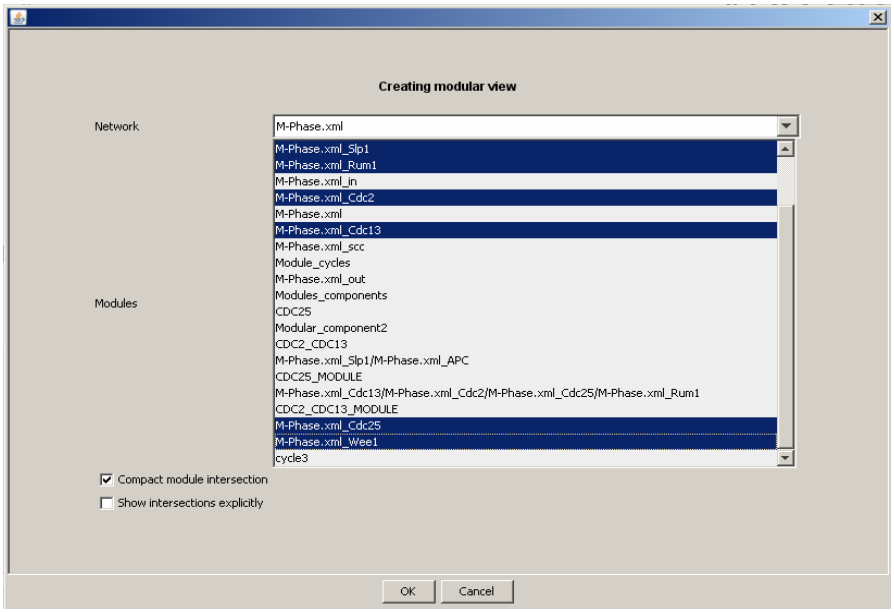
\includegraphics[width=0.8\textwidth]{graphics/Modular_view_Pop-up_window}
%\caption{BiNoM modular view of the newtork: Pop-up window in which the initial graph and the modules are specified. }
%\label{Modular_view_Pop-up_window}
%\end{figure}
%\\There are different types of modular views. The modules are connected by: (1) the number of shared interactions (figure~\ref{Modular_view_The_resulting_modular_network}, upper panel); (2) the number of shared nodes (reactions + species) for which case the box “Compact module intersection” must be checked (figure~\ref{Modular_view_The_resulting_modular_network}, middle panel); and (3) the shared nodes and reactions showed explicitly (figure~\ref{Modular_view_The_resulting_modular_network}, lower panel).
%\begin{figure}
%\centering
%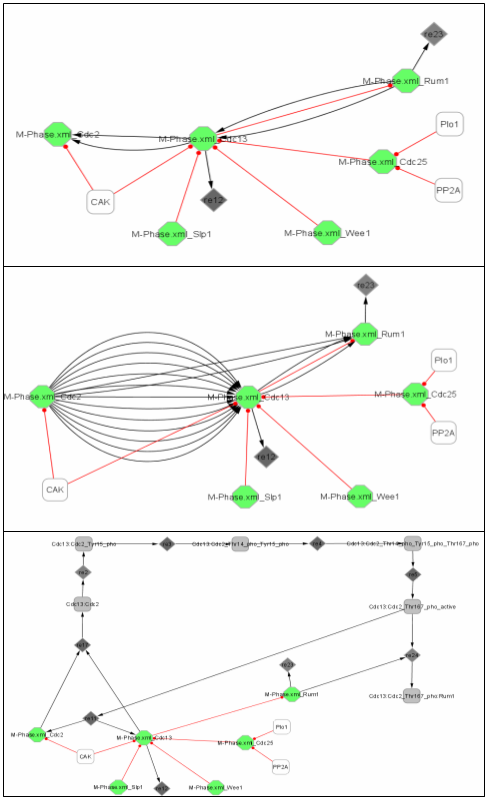
\includegraphics[width=0.8\textwidth]{graphics/Modular_view_The_resulting_modular_network}
%\caption{BiNoM modular view of the newtork: The resulting modular network (upper panel) with compact module intersections (middle panel) and with explicit intersections (lower panel).}
%\label{Modular_view_The_resulting_modular_network}
%\end{figure}

\subsection{Cluster Networks}
\textbf{Plugins$\Rightarrow$BiNoM 2.1$\Rightarrow$BiNoM Analysis$\Rightarrow$Cluster networks}\\
This command lumps together the modules that share a certain proportion of nodes. At a first glance, it can easily be concluded from Figure~\ref{Modular_view_The_resulting_modular_network} (middle panel) that, for example, the modules M-Phase.xml\_Cdc13 and M-Phase.xml\_Cdc2 share a lot of proteins or protein complexes. Therefore, we can assume that these two modules will collapse into one big module. To determine the clusters, the intersection threshold can be set (from 0 to 100\% intersecting components). For a 30\% intersection threshold, Figure~\ref{Clusters_of_modules_using_the_material_decomposition} is obtained. Four clusters of modules were proposed and linked.\\\\
An alternative modular view has been obtained using the cycle decomposition instead of the material decomposition. The cycles are presented in Figure~\ref{Minimal_cycle_decomposition_of_the M-Phase}. They are obtained by clustering the three cycles into two (cycle 1 + cycle2/cycle3) and organized into a modular view (Figure~\ref{Clusters_of_modules_using_the_cycle_decomposition}).\\
\begin{figure}
\centering
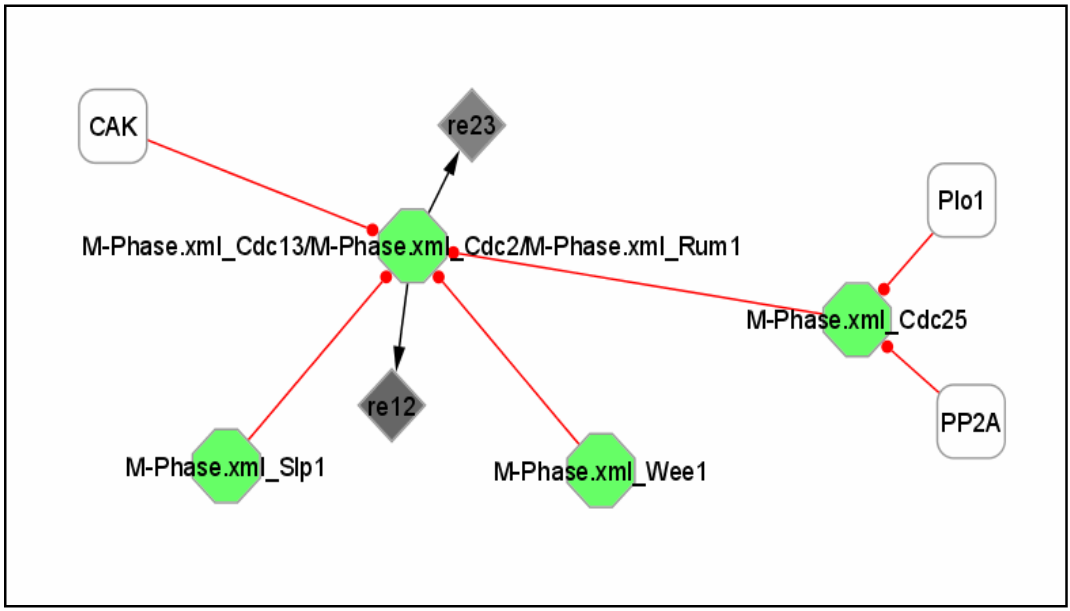
\includegraphics[width=0.8\textwidth]{graphics/Clusters_of_modules_using_the_material_decomposition}
\caption{Clusters of modules. The obtained diagram is a compact modular view of the M-Phase network using the material decomposition and material components clustering}
\label{Clusters_of_modules_using_the_material_decomposition}
\end{figure}
\begin{figure}
\centering
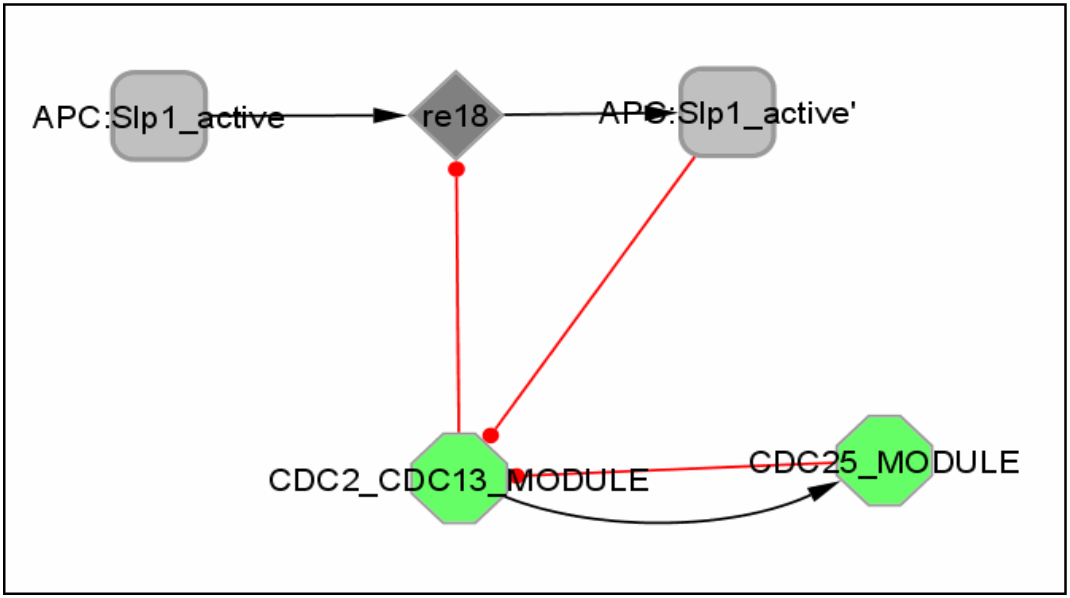
\includegraphics[width=0.8\textwidth]{graphics/Clusters_of_modules_using_the_cycle_decomposition}
\caption{Clusters of modules. The obtained diagram is a compact modular view of the M-Phase network using the relevant cycle decomposition and cycle clustering}
\label{Clusters_of_modules_using_the_cycle_decomposition}
\end{figure}

\subsection{Mono-molecular react.to edges}
\textbf{Plugins$\Rightarrow$BiNoM 2.1$\Rightarrow$BiNoM Analysis$\Rightarrow$Mono-molecular react. to edges}\\
This function transforms monomolecular reaction nodes (i.e. reactions with one
reactant and one product) into ‘influence’ edges. Thus, monomolecular (linear)
reactions are represented as edges and the reaction graph is not bi-partite
anymore. When the reaction nodes have the type of influence specified (through
the Cytoscape ‘EFFECT’ attribute), the graph is transformed automatically into an
influence graph (see Figure~\ref{Network_to_influence_graph}: upper panel:
BioPAX network, lower panel, the equivalent influence network). Non-linear
non-monomolecular reactions (such as complex assemblies) are not transformed and
remain to be represented as network nodes.
\begin{figure}
\centering
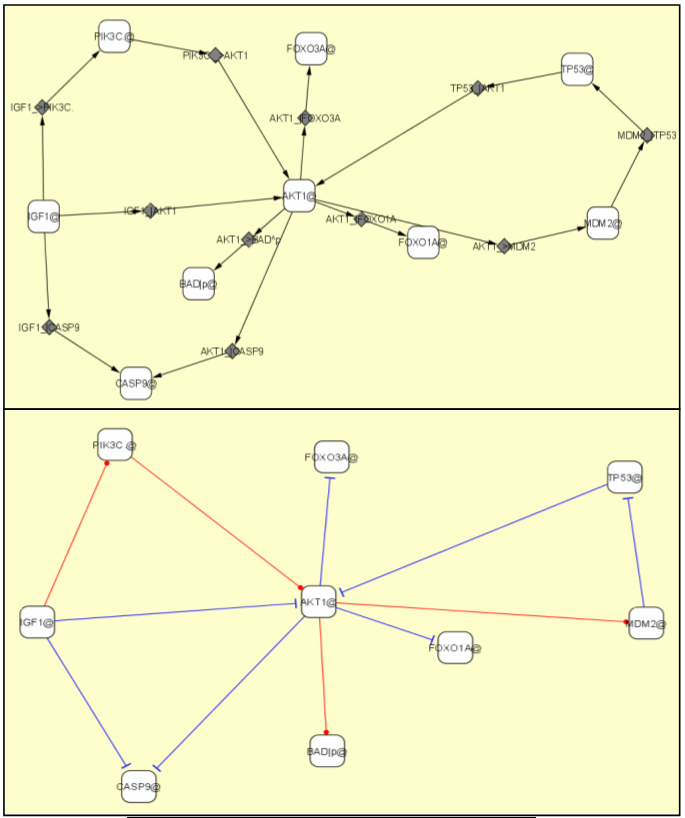
\includegraphics[width=0.8\textwidth]{graphics/Network_to_influence_graph}
\caption{From a BioPAX network (upper panel) to an influence graph (lower panel).}
\label{Network_to_influence_graph}
\end{figure}

\subsection{Linearize network}

%Remove reactions and reconnect edges according to a supposed influence (figure~\ref{Linearized_Network_M-Phase})\\
%\includegraphics[width=20pt,height=20pt]{graphics/warning} The got network is not an influence network in the biological sense. But, it can be used to build an influence network.
%\begin{figure}
%\centering
%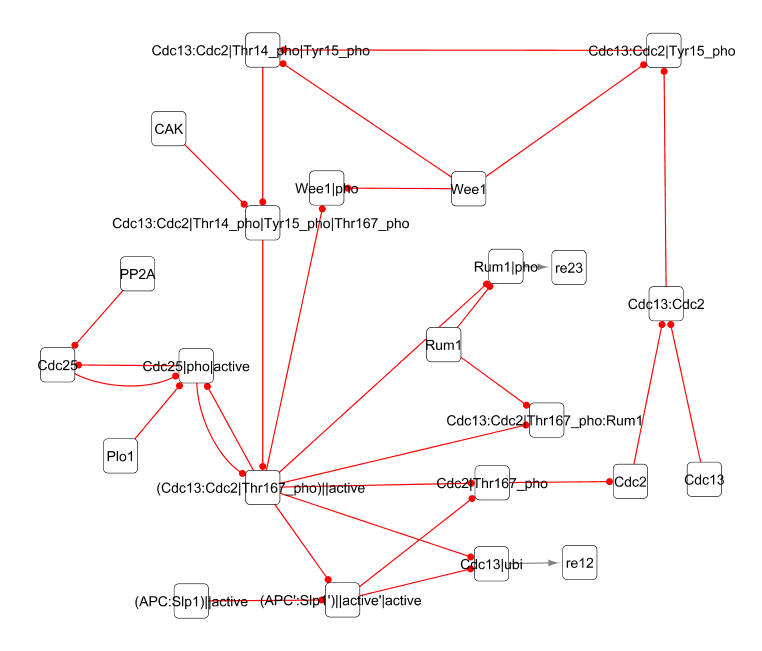
\includegraphics[width=0.8\textwidth]{graphics/Linearized_Network_M-Phase}
%\caption{Result of applying "Linearize network" to M-Phase.}
%\label{Linearized_Network_M-Phase}
%\end{figure}
The ``linearization'' replaces explicit reactions of complex formation by direct influences between constituents and complexes (in the case of an influence network imported from an AIN file).

To illustrate this function, import the AIN file \textit{cell\_cycle\_AIN.txt}.

\textbf{Plugins$\Rightarrow$BiNoM 2.1$\Rightarrow$BiNoM I/O$\Rightarrow$Import influence network from AIN file...}\\
Click two times 'OK' for the specification of the families. A new network is created. Then, apply the linearization functions
\textbf{Plugins$\Rightarrow$BiNoM 2.1$\Rightarrow$BiNoM Analysis$\Rightarrow$‘Linearize’ network}\\

A new 'linearized' network is created (figure ~\ref{Linearized_Network_Cell_Cycle}).

\begin{figure}
  \centering
  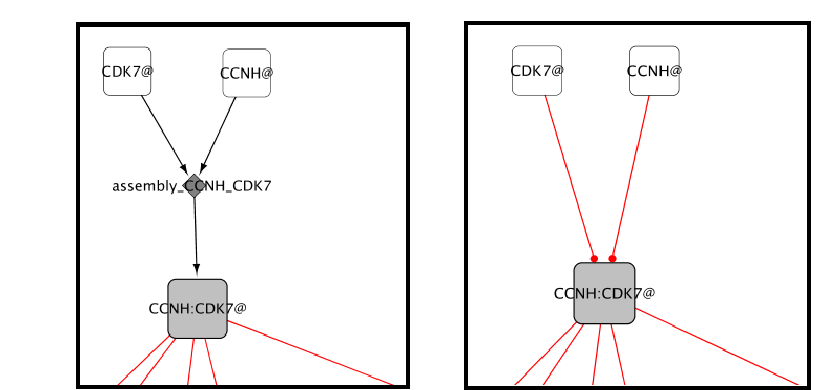
\includegraphics[width=0.8\textwidth]{graphics/linearize_cc.pdf}
  \caption{Example of explicit reaction of complex formation (left panel) that can be replaced by direct connections (right panel) using the ``linearization`` function of BiNoM.}
  \label{Linearized_Network_Cell_Cycle}
\end{figure}


\subsection{Exclude intermediate nodes}
\textbf{Plugins$\Rightarrow$BiNoM 2.1$\Rightarrow$BiNoM Analysis$\Rightarrow$Exclude intermediate nodes}\\
This function opens a dialog where nodes to be excuded can be selected (figure~\ref{Exclude_nodes_Dialog}). It creates a network without the selected nodes and reconnects edges.
\begin{figure}
\centering
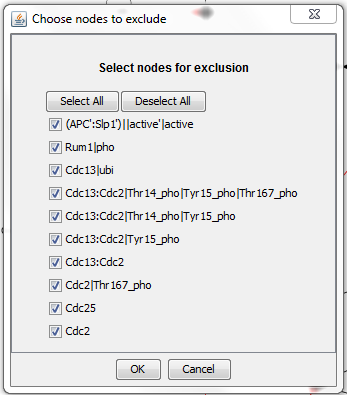
\includegraphics[width=7 cm]{graphics/Exclude_nodes_Dialog}
\caption{Dialog to select nodes to be excluded in the created network.}
\label{Exclude_nodes_Dialog}
\end{figure}

\subsection{Extract Reaction Network}
\textbf{Plugins$\Rightarrow$BiNoM 2.1$\Rightarrow$BiNoM Analysis$\Rightarrow$Extract reaction networks}\\
This function cleans up the diagram to only keep the reaction network. Only nodes with ‘XXXX\_REACTION’ and ‘XXXX\_SPECIES’ attributes (where XXXX stands for any word) are kept as a result of this operation. For example, it helps to clean the reaction network interface from the result of querying BioPAX index (which contains many other node types such as entities and publications.

\subsection{Path Influence Quantification analysis}
\textbf{Plugins$\Rightarrow$BiNoM 2.1$\Rightarrow$BiNoM Analysis$\Rightarrow$Path Influence Quantification analysis}\\

%This function is based on an algorithm of  Path Influence Quantification
%(PIQuant). Shortly, for every annotated nodes, the influence is computed by
%summing (optimal and sub-optimal) paths contribution (1/(length of the path)),
%multiplied by the nodes annotation that represent biological data. For global
%influence computation, influences are summed on all over the annotated nodes.
%The figure \ref{PIQuant_example} shows the computing in a simple example.\\\\

This function calculates a score to quantify the effect of experimental data
onto one or more target nodes for a given network architecture, named the
PIQuant score (Pathway Influence Quantification). The target node can be a gene
or a phenotype of interest (such as cell cycle or apoptosis). We define as
annotated nodes any node of the network for which we have experimental data
available. The experimental data can be for instance an mRNA expression value
(ratio disease/normal). We also assume that we have determined all the paths
from the annotated nodes to the target nodes using an appropriate algorithm
(such as Dijkstra's shortest paths algorithm). The PIQuant score is then defined as:


$$
 PIQuant_{Score} = \sum_{k=1}^{q} \alpha_{k} \sigma_{k} \frac{1}{\lambda_{k}}
$$

 A path $k \in \{1,\ldots , q\}$ is defined
as a the sequence of consecutive connected nodes
between a source node and a target node (without repetition of any node
or edge).

The annotation $\alpha_k$ of the path $k$ is defined as the annotation (real value representing the experimental data) 
of its source node. We define the sign $\sigma_k$
of the path $k$ as the product of the signs of every edge of the path and finally
the length $\lambda_k$ of the path $k$ as the number of edges in the path. We
hypothesize that the longer the path is, the lesser the global influence will be
on the target node.

\includegraphics[width=20pt,height=20pt]{graphics/warning} The Cytoscape edge attribute
which encodes the influence corresponding to the sign (+1 or -1) of the edge is "EFFECT" which can take 2 values EFFECT:activation and
EFFECT:inhibition.\\\\

\begin{figure}
  \centering
  %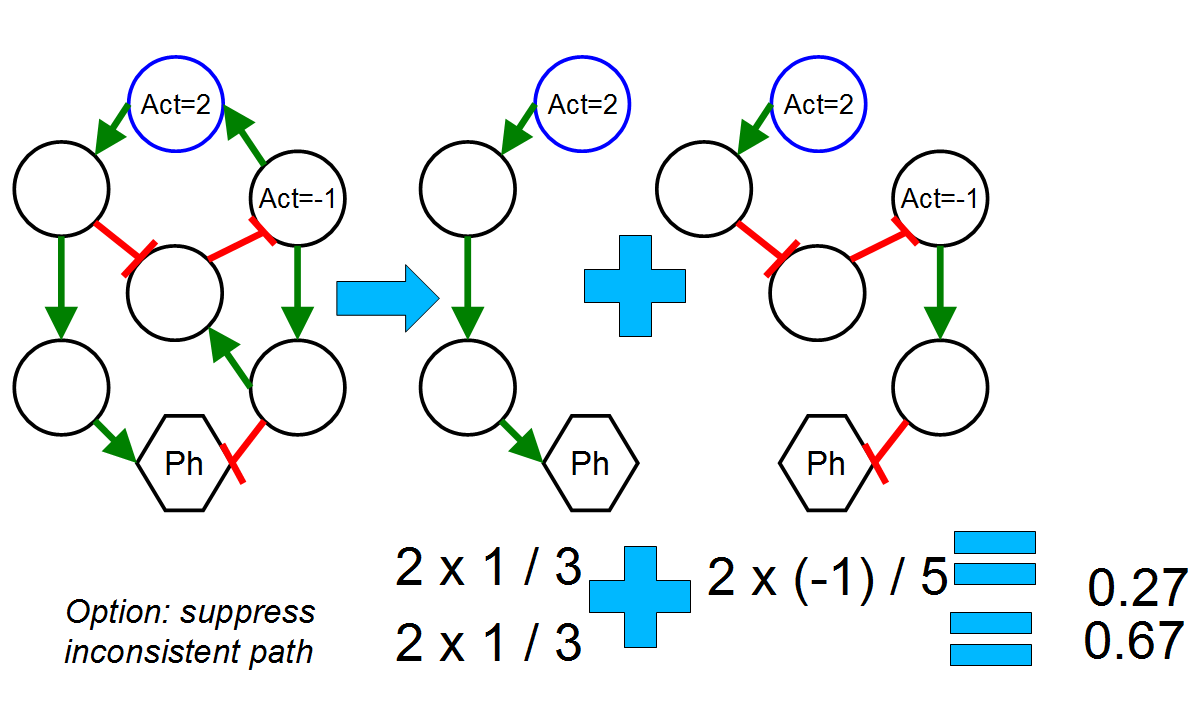
\includegraphics[width=0.8\textwidth]{graphics/PIQuant_example}
  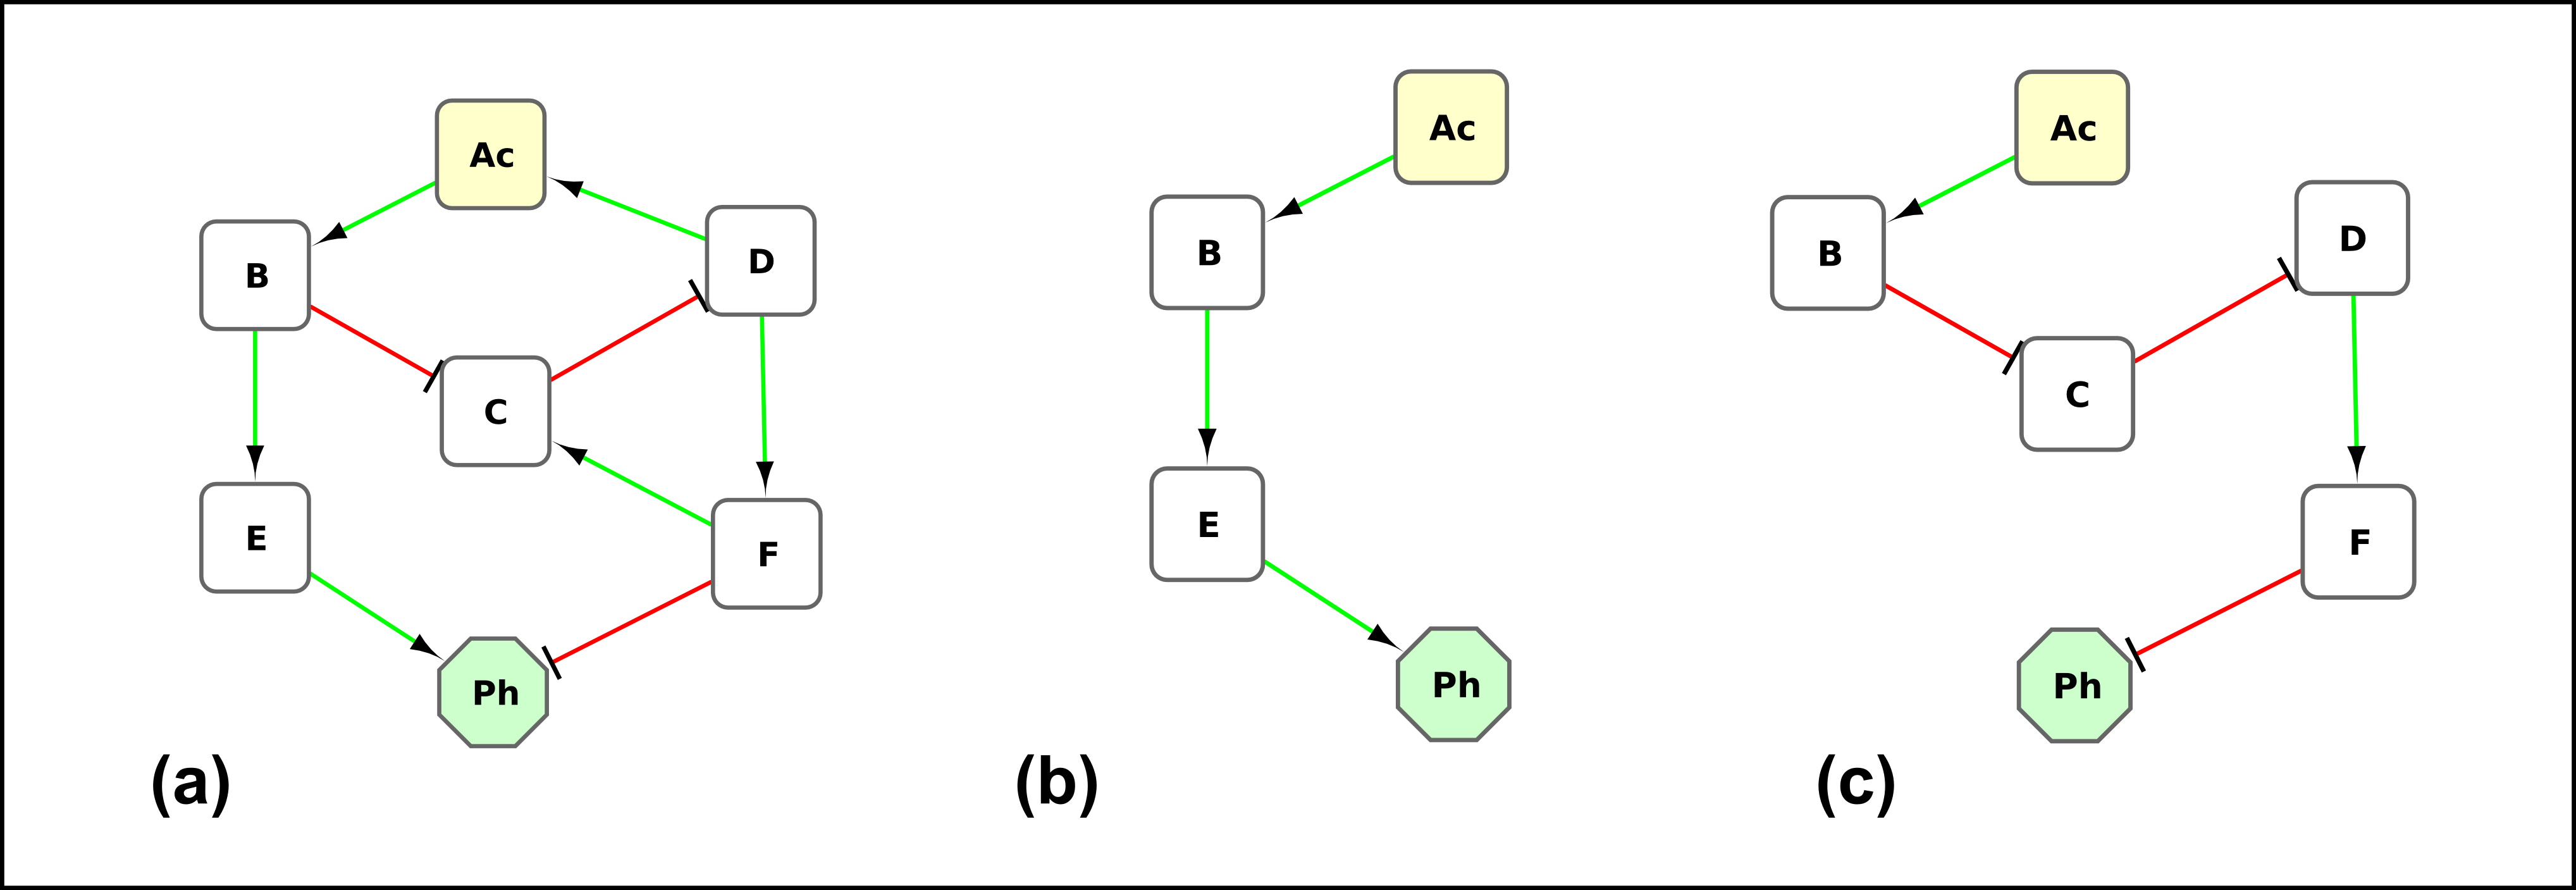
\includegraphics[width=0.8\textwidth]{graphics/piquant_networks}
  \caption{A simple influence network. The network is composed of seven nodes
and nine edges (a). The two paths (b,c) extracted from this network start from
the source node \textbf{Ac} and end at the target node \textbf{Ph} (a phenotype of interest). The
nodes \textbf{Ac} and \textbf{D} are annotated using experimental data, and have the values 2.0
and -1.0 respectively.}
  \label{PIQuant_example}
\end{figure}


In the case of the network presented in figure~\ref{PIQuant_example}a, let us
consider Ac the source node and Ph the target node and consider only the two
paths defined in the figure~\ref{PIQuant_example}b and
figure~\ref{PIQuant_example}c. Given that the
node Ac is annotated by the value $2.0$, that the first path has a length
equal to 3, and that the second path has a length equal to 5, we can calculate the PIQuant score
of the node Ac to the node Ph as:

$$
 PIQuant_{Score} = 2 \cdot 1 \cdot \frac{1}{3} + 2 \cdot (-1) \cdot \frac{1}{5}
= 0.27
$$


Sometimes a path has one or more intermediate nodes that are annotated nodes
(i.e. for which we have experimental data values),
in addition to the source node.
In that case, the intermediate node is \textit{consistent} if the sign of its
annotation is the same as the sign of the source node annotation multiplied by
the sign of the
path from the source node to the intermediate node. If signs are opposite, the
node is \textit{inconsistent}.
A path is \textit{consistent} if each annotated intermediate nodes is
consistent. A path is \textit{inconsistent} if at least one intermediate node is
\textit{inconsistent}.
In other words, a path is inconsistent when the
sign of the experimental data value for a node is opposite to the sign
of the path.

For example, according to the network represented in figure~\ref{PIQuant_example}c, there is an influence from Ac to Ph
that goes through D . But if this path
is functional, the annotation of node D should have the same sign as the annotation for node Ac, because
Ac activates D indirectly (i.e. the path from Ac to D has a positive sign). In this case, the sign of D annotation (the experimental value) is opposite to
the sign of Ac annotation, and therefore, the path from Ac to Ph that goes through D is inconsistent.

Practically, we offer the option to
keep or not the inconsistent paths for the calculation of the PIQuant score,
depending on how the user wants to analyze the calculations. An inconsistent
path could indicate that the path is not complete, or could also indicate that
the path is correct but not active under the precise conditions in which the
experimental data was generated, corresponding to a different context.

In the case mentionned above in figure~\ref{PIQuant_example}c, if only consistent paths are kept, then the PIQuant score of Ac to Ph
becomes:

$$
 PIQuant_{Score} = 2 \cdot 1 \cdot \frac{1}{3} = 0.67
$$

This score is higher than the value previously obtained with all the paths, and can be interpreted in this case as a higher activation of the phenotype.


In order to calculate the PIQuant score, an influence network with annotated
nodes should be created, for example using the AIN file format (see the AIN file
format description in the appendix).

One the network is created in Cytoscape, then we can call the BiNoM function to calculate the PIQuant score.

\textbf{Plugins$\Rightarrow$BiNoM 2.1$\Rightarrow$BiNoM Analysis$\Rightarrow$Path Influence Quantification analysis}\\

%For global influences, a p-value can be computed, by shuffling the annotation.
%Among the possible options accessible in BiNoM, the possibility of removing
%inconsistent path (paths that have an intermediate node with inconsistent
%annotation) was sometimes used.\\\\

This function has two dialogs, one for choosing the annotated nodes, targets nodes and path search algorithm, and one to display the results of the calculation.

Step 1 see figure~\ref{Path_consistency_analyser_Dialog1}:

\begin{itemize}
  \item Select the attribute name corresponding to the annotation and click update list, only active nodes are
  displayed in box.
  \item Select target nodes.
  \item Choose one algorithm for path searching, see glossary in section \ref{GLOSSARY} for details on the different algorithms.
  \item Click OK.
\end{itemize}

\begin{figure}
  \centering
  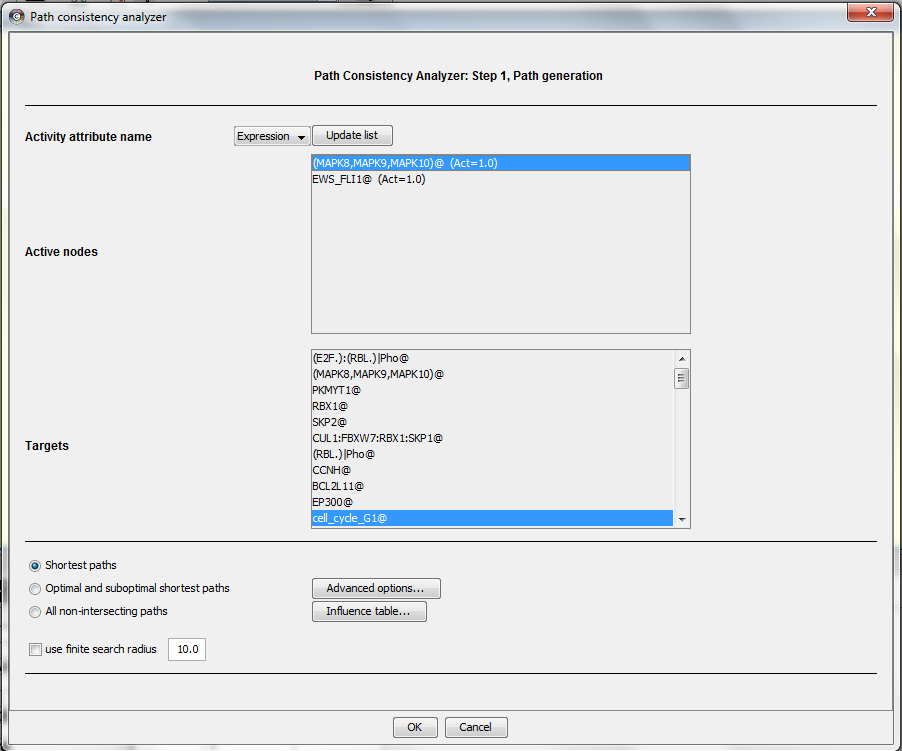
\includegraphics[width=0.8\textwidth]{graphics/Path_consistency_analyser_Dialog1}
  \caption{Path consistency analysis: dialog of step 1, select annotated nodes,
targets and the algorithm for searching the paths.}
  \label{Path_consistency_analyser_Dialog1}
\end{figure}

The step 2 dialog (the results of the PIQuant score calculations) is displayed on figure~\ref{Path_consistency_analyser_Dialog2}.



\begin{figure}
  \centering
  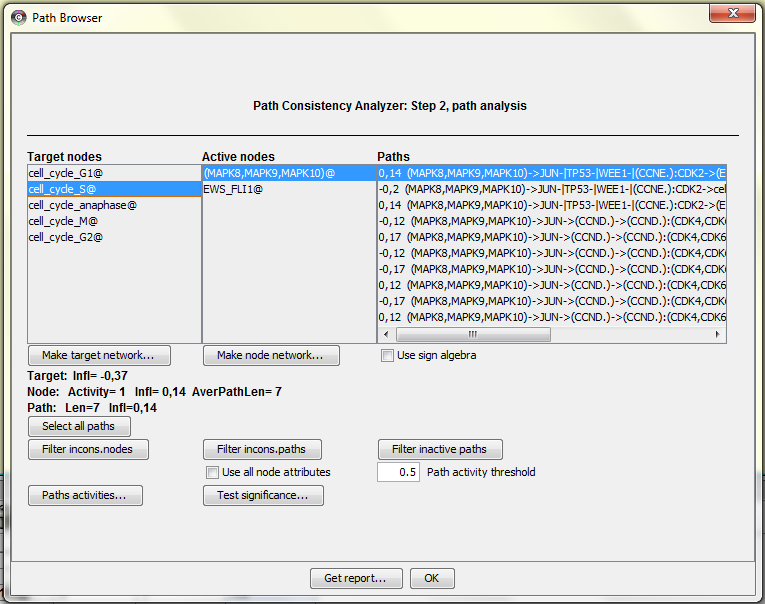
\includegraphics[width=0.8\textwidth]{graphics/Path_consistency_analyser_Dialog2}
  \caption{Path consistency analysis: dialog of step 2, display paths and
activities, get all results}
  \label{Path_consistency_analyser_Dialog2}
\end{figure}  

%\subsection{OCSANA analysis}
%\textbf{Plugins$\Rightarrow$BiNoM 2.1$\Rightarrow$BiNoM Analysis$\Rightarrow$OCSANA analysis}\\
%Work in progress.

\subsection{Create neighborhood sets file}
\textbf{Plugins$\Rightarrow$BiNoM 2.1$\Rightarrow$BiNoM Analysis$\Rightarrow$Create neighborhood sets file}\\
This function creates a file *.gmt (a text file where nodes are separated by \textless Tab\textgreater) containing the neighbors of selected nodes according to option of the dialog(figure~\ref{Create_Neigborhood_File_Dialog})
\begin{figure}
\centering
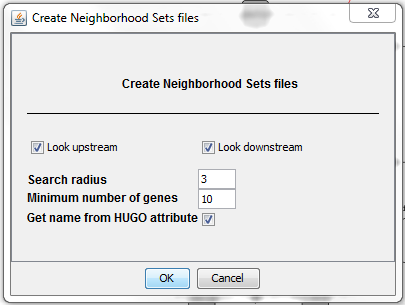
\includegraphics[width=7 cm]{graphics/Create_Neigborhood_File_Dialog}
\caption{Diialog for options of creating a neighborhood sets file.}
\label{Create_Neigborhood_File_Dialog}
\end{figure}  

\clearpage
\section{BiNoM Module Manager}
Module manager is useful for creating modular view of large networks without loosing details of modules (using “nest”, object of Cytoscape v7 and after).

\subsection{Create Network of Modules}
\textbf{Plugins$\Rightarrow$BiNoM 2.1$\Rightarrow$BiNoM Module Manager$\Rightarrow$Create Network of Modules}\\
Create a new network from a list of sub-networks (sub-networks are selected in the network list see figure~\ref{Create_network_of_modules}).\\
Nodes=modules, no edge. Visual style created in VizMapper for module network . The got network is as \ref{M-Phase_Material_Modular} without edge and with nodes on grid.\\
\includegraphics[width=20pt,height=20pt]{graphics/warning} Module names and node names must be different, all network names too.\\\\
To go from module to sub-network:\\
select node$\Rightarrow$CRight click$\Rightarrow$CNested Network$\Rightarrow$Go to Nested Network.
\begin{figure}
\centering
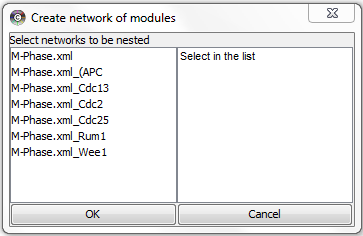
\includegraphics[width=0.8\textwidth]{graphics/Create_network_of_modules}
\caption{Dialog for select networks to become modules in modular0}
\label{Create_network_of_modules}
\end{figure}

\subsection{Create Connections between Modules}
\textbf{Plugins$\Rightarrow$BiNoM 2.1$\Rightarrow$BiNoM Module Manager$\Rightarrow$Create Connections between Modules}\\
Create edges linking modules from all edges of the selected network.\\
Links are simplified, no distinction between left and right (molecule flow), no duplication if same interaction.\\
Warning message if duplicated or absent nodes (may disturb links).
\begin{figure}
\centering
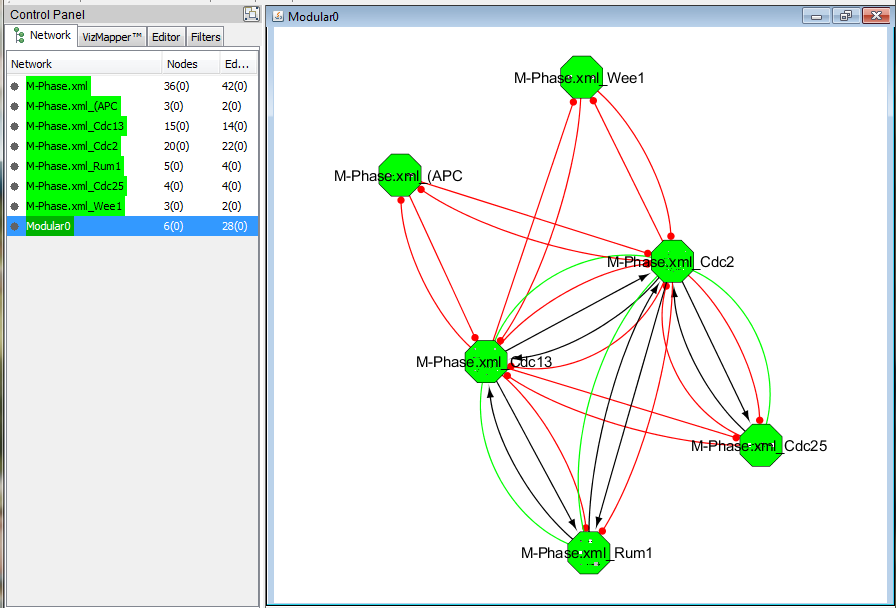
\includegraphics[width=0.8\textwidth]{graphics/M-Phase_Material_Modular}
\caption{M-Phase is divided into modules by get material component. The modular view is got by creating network of modules with organic layout. The function "Create connections between modules" links modules according to the reference network. The function "Find common nodes in modules" creates intersection edges. }
\label{M-Phase_Material_Modular}
\end{figure}

\subsection{Create Modules from Networks}
\textbf{Plugins$\Rightarrow$BiNoM 2.1$\Rightarrow$BiNoM Module Manager$\Rightarrow$Create Modules from Networks}\\
Create modules in the active network from a list of sub-networks (sub-networks are selected in the network list)\\
All edges are kept. See edge attribute PREVIOUS\_ID for their origin.\\
The attribute BIOPAX\_NODE\_TYPE is set to “pathway” (see visual style BiNoM BioPAX).\\
\includegraphics[width=20pt,height=20pt]{graphics/warning} All nodes of sub-networks must be found once in the active network (no intersection between sub-networks).

\subsection{Agglomerate the Nearest Nodes in Modules}
\textbf{Plugins$\Rightarrow$BiNoM 2.1$\Rightarrow$BiNoM Module Manager$\Rightarrow$Agglomerate the Nearest Nodes in Modules}\\
Create modules and a modular view by agglomerating the nearest nodes in the active network (see~algorithm~in section~\ref{Agglomeration_by_shortest_path}.\\\\
Input 2 parameters to get not too big sub-networks containing not too far nodes:
\begin{itemize}
\item Maximal distance between nodes or modules in number of edges,
\item Maximal number of nodes in modules.
\end{itemize}
Confirm creation if agree with displayed result (see dialog~\ref{Agglomerate_in_modules_dialog}).\\\\
Sub-networks are created and gathered in a packed network as the function "Create modules from networks" (see figure~\ref{M-Phase_packed}).
\begin{figure}
\centering
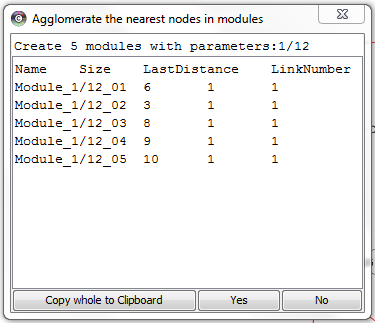
\includegraphics[width=0.8\textwidth]{graphics/Agglomerate_in_modules_dialog}
\caption{This window displays modules, number of node, last distance and number of links of agglomerating process. Yes lauches the process of agglomerating.}
\label{Agglomerate_in_modules_dialog}
\end{figure}
\begin{figure}
\centering
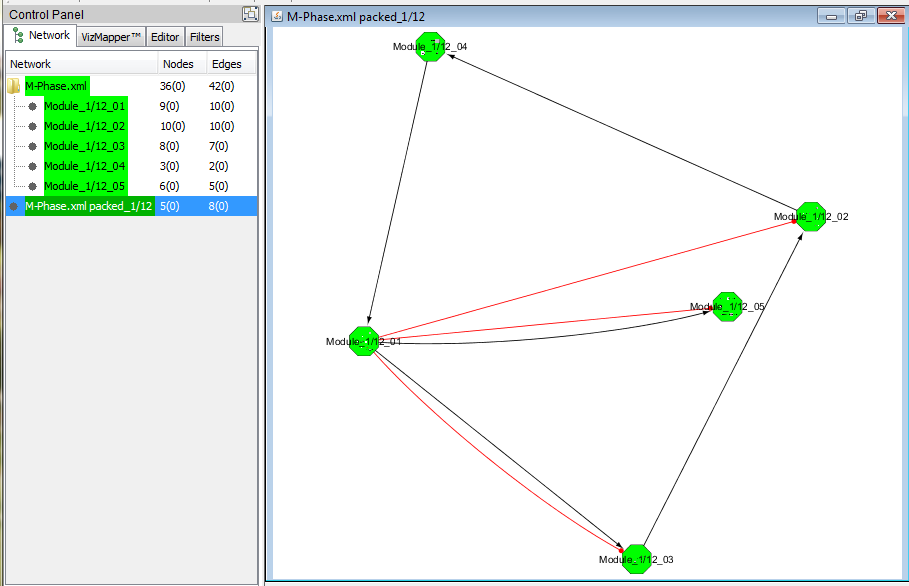
\includegraphics[width=0.8\textwidth]{graphics/M-Phase_packed}
\caption{M-Phase is got by creating network from modules, modules created by agglomerating the nearest nodes (maximal distance=1, maximal size=12 nodes).}
\label{M-Phase_packed}
\end{figure}

\subsection{List Nodes of Modules and Network}
\textbf{Plugins$\Rightarrow$BiNoM 2.1$\Rightarrow$BiNoM Module Manager$\Rightarrow$List Nodes of Modules and Network}\\
List nodes of network and nodes included in modules.\\
Result in text box can be simply copied in a spreadsheet through clipboard.

\subsection{Find Common Nodes in Modules}
\textbf{Plugins$\Rightarrow$BiNoM 2.1$\Rightarrow$BiNoM Module Manager$\Rightarrow$Find Common Nodes in Modules}\\
Display in text box the belonging matrix of nodes (modules in columns, nodes in rows, size of modules in last row, frequency in modules in last column); result more easily usable after copying in a spreadsheet (see~\ref{Common_nodes_in_modules}.\\\\
Create intersection edges with number of common nodes as attribute (COMMON\_NODES), green edges in figure~\ref{M-Phase_Material_Modular}.\\\\
Create node attribute containing the node numbers of modules (NODE\_NUMBER).\\\\
Module Visual StyleCan be adapted to the wished visual aspect by hands in VizMapper, for example:
\begin{itemize}
\item To visualize NODE\_NUMBER: double click Node Size, select NODE\_NUMBER, continuous mapping, adjust width by graphical view.
\item To visualize COMMON\_NODES double click Edge Line Width, select COMMON\_NODES, continuous mapping, adjust width by graphical view.
\end{itemize}
\begin{figure}
\centering
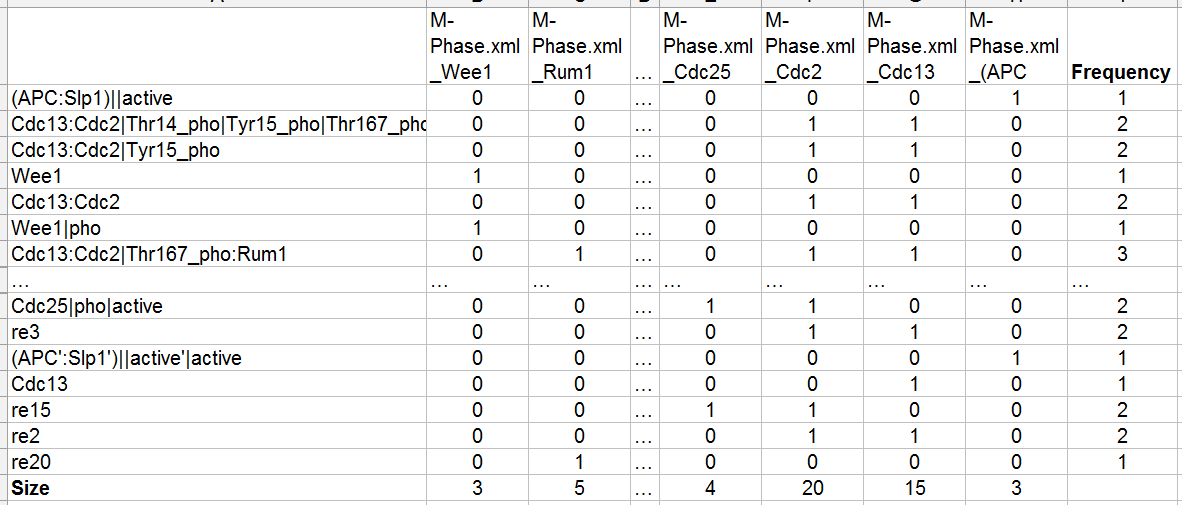
\includegraphics[width=0.8\textwidth]{graphics/Common_nodes_in_modules}
\caption{Matrix of nodes: modules in columns, nodes in rows, size of modules in last row, frequency in modules in last column.}
\label{Common_nodes_in_modules}
\end{figure}

\subsection{Assign Module Names to Node Attribute}
\textbf{Plugins$\Rightarrow$BiNoM 2.1$\Rightarrow$BiNoM Module Manager$\Rightarrow$Assign Module Names to Node Attribute}\\
Create a node attribute (named as the modular network), containing module names. This attribute may be used to visualize modules in the reference network.

\subsection{List Components of Species in Network and Modules}
\textbf{Plugins$\Rightarrow$BiNoM 2.1$\Rightarrow$BiNoM Module Manager$\Rightarrow$List Components of Species in Network and Modules}\\
List components of species (their names must respect BiNoM syntax). Useful to name modules.

\subsection{Create Network from Union of Selected Modules}
\textbf{Plugins$\Rightarrow$BiNoM 2.1$\Rightarrow$BiNoM Module Manager$\Rightarrow$Create Network from Union of Selected Modules}\\
Create a network from union of selected modules and its corresponding module in the current network (named by module names separated by \&).

\subsection{Create Network from Intersection of 2 Selected Modules}
\textbf{Plugins$\Rightarrow$BiNoM 2.1$\Rightarrow$BiNoM Module Manager$\Rightarrow$Create Network from Intersection of 2 Selected Modules}\\
Create a network from intersection of 2 selected modules and its corresponding module (named by module names separated by \textbar.\\\\
Confirm for deleting the common nodes in the selected modules.

\subsection{Recreate Lost Connections inside Modules}
\textbf{Plugins$\Rightarrow$BiNoM 2.1$\Rightarrow$BiNoM Module Manager$\Rightarrow$Recreate Lost Connections Inside Modules}\\
Recreate connections inside modules which may have been lost by modularizing operations.

\subsection{Destroy Networks Unused as Module}
\textbf{Plugins$\Rightarrow$BiNoM 2.1$\Rightarrow$BiNoM module manager$\Rightarrow$Destroy Networks Unused as Module}\\
Select networks to be deleted among a list of networks which are not used as modules in the current network (simplify cleaning session).

\clearpage
\section{BiNoM BioPAX3 Utils}
\subsection{BioPAX 3 Property Editor} \label{BioPAX_Property_Editor}
\textbf{Plugins$\Rightarrow$BiNoM 2.0$\Rightarrow$BiNoM BioPAX 3 Utils$\Rightarrow$ BioPAX 3 Property Editor}\\

All the information available in a BioPAX file can be easily retrieved using the
BioPAX Property Editor function. A component on the diagram must be selected
first (CDC2 in Figure \ref{BioPAX_Property_Editor_cdc2}) and a window appears
with all available information concerning the molecule.\\\\

\begin{figure}[h]
\centering
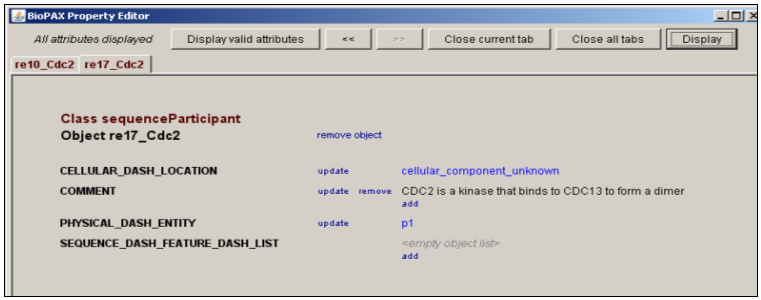
\includegraphics[width=0.8\textwidth]{graphics/BioPAX_Property_Editor_cdc2}
\caption{BioPAX Property Editor: example of the properties concerning CDC2
component in M-Phase model}
\label{BioPAX_Property_Editor_cdc2}
\end{figure}


\parbox{\textwidth}{ In the menu of the Property Editor, several options are
offered:

\begin{itemize}
\item Display valid attributes / Display all attributes hides all the empty
fields (for example, in Figure \ref{BioPAX_Property_Editor_apoptosis}:
Availability or Evidence have \textless empty object list\textgreater and would
be hidden) / shows all the available fields, even the empty ones.
\item  \textless\textless~and \textgreater\textgreater~correspond to back or
forward buttons and follow the historical exploration of the Property Editor
(similar to ‘Back’ and ‘Forward’ buttons of a network browser).
\item Close current tab or Close all tabs closes the current page of the
property editor or all the open pages.
\item  Display / Edit shows a simple display of the page editor where no change
can be made (Figure \ref{BioPAX_Property_Editor_apoptosis}) / allows changes in
the fields by adding, removing or updating information (Figure
\ref{BioPAX_Property_Editor_cdc2}). For the latter, click first on the Edit tab
on the upper menu, then on update situated near the field to modify. In Figure
\ref{BioPAX_Property_Editor_cdc2}, as an example, some comments were added
manually: “CDC2 is a kinase that binds to CDC13 to form a dimer”. In the
Apoptosis example (Figure \ref{BioPAX_Property_Editor_apoptosis}), extensive
information is already available concerning the pathway, references, etc.
\end{itemize}}
\begin{figure}[h]
\centering
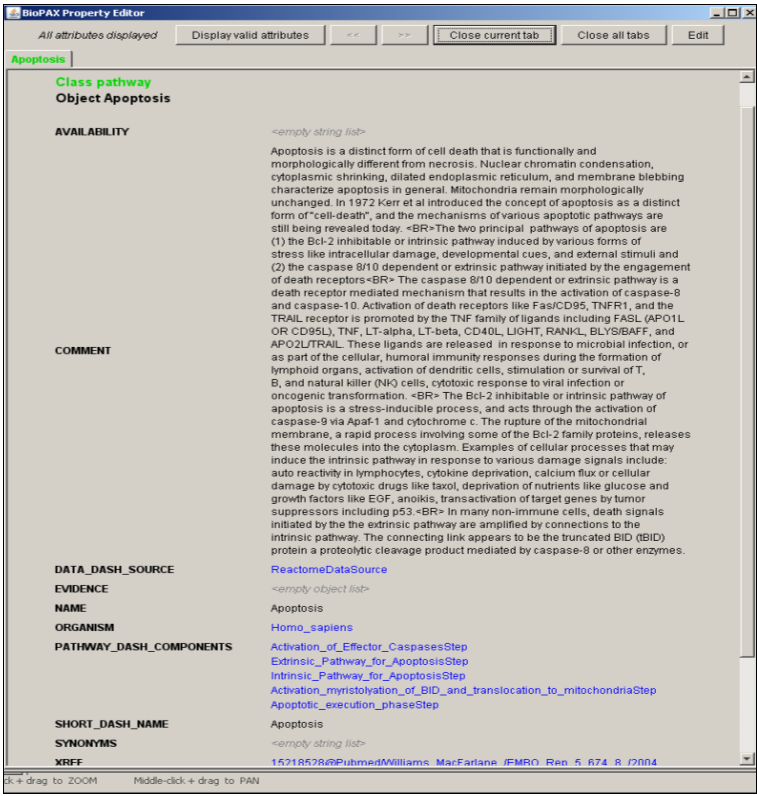
\includegraphics[width=0.8\textwidth]{graphics/BioPAX_Property_Editor_apoptosis}
\caption{BioPAX Property Editor: example of “apoptosis pathway” node properties}
\label{BioPAX_Property_Editor_apoptosis}
\end{figure}	
For more details on BioPAX description standard, visit the webpage:
http://www.biopax.org/ 
\subsection{BioPAX 3 Class Tree}
\textbf{Plugins$\Rightarrow$BiNoM 2.0$\Rightarrow$BiNoM BioPAX 3 Utils$\Rightarrow$BioPAX 3 Class
Tree}\\
All the statistics concerning the pathway are listed: the number of reactions,
associations or catalyses, the number of proteins or complexes, etc
(figure~\ref{BioPAX_Class_Tree}). More information can be accessed by selecting
a specific object which, when clicked on, leads to the BioPAX 3 Property Editor
window (see section~\ref{BioPAX_Property_Editor}).\\\\
\begin{figure}[h]
\centering
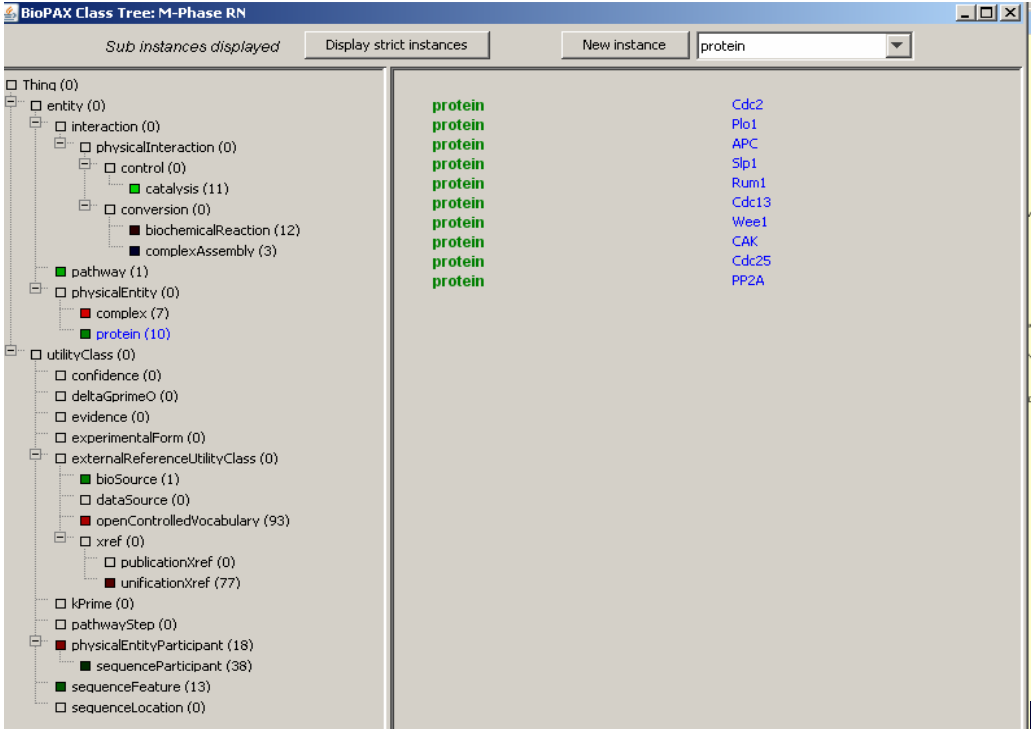
\includegraphics[width=0.8\textwidth]{graphics/BioPAX_Class_Tree}
\caption{BioPAX Class tree. On the left frame, the model is described in terms
of interactions, entities, etc. On the right frame, the proteins, selected in
the left frame, are listed. The links are clickable and open a BioPAX Property
Editor window.}
\label{BioPAX_Class_Tree}
\end{figure}
To complete the network, the user can easily add new information or a new
protein, protein complex, type of interaction, etc., by clicking on the New
Instance tab.

\subsection{Use Simplified URI Names}
\textbf{Plugins$\Rightarrow$BiNoM 2.0$\Rightarrow$BiNoM BioPAX 3 Utils$\Rightarrow$Use Simplified URI Names}\\

In the BioPAX Class Tree, protein names can have either URI names (Uniform Resource Identifier used to give a unique identification to proteins) or “BiNoM Naming Service” names. For example, for the apoptosis pathway, the protein BAD is referred to as\\

“\textit{UniProt\_Q92934\_Bcl2\_antagonist\_of\_cell\_death\_BAD\_\_Bcl\_2\_binding\_component\_6\_\_Bcl\_\_XL\_Bcl\_2\\
\_associated\_death\_promoter\_\_Bcl\_2\_like\_8\_protein}”\\

in the URI case and just “BAD” in the BiNoM Naming Service case. For the rules of how BiNoM generates names see section~\ref{BiNoM_Naming_Service}.

\subsection{Synchronize networks with BioPAX 3}
\textbf{Plugins$\Rightarrow$BiNoM 2.0$\Rightarrow$BiNoM BioPAX 3 Utils$\Rightarrow$Synchronize networks with BioPAX 3}\\
This command updates all the interfaces according to the changes made to individual BioPAX objects.
\clearpage
\section{BiNoM BioPAX3 Query}
\begin{figure}[h]
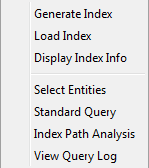
\includegraphics{graphics/BiNoM_BioPAX3_Query}
\end{figure}
\clearpage
\section{BiNoM Utilities}
\begin{figure}[h]
\includegraphics{graphics/BiNoM_Utilities}
\end{figure}
\clearpage
\section{Appendices}
\subsection{Attributed graph model}\label{Attributed_graph_model}
BiNoM manipulates the information contained in the standard systems biology files by mapping it onto a labeled graph, called index. The index does not try to map the totality of all details; it rather serves as a connection map for the objects contained in other ontologies such as BioPAX. In other words, the index contains the minimum information needed to graphically represent objects and connections between them. Index elements (nodes and edges) are annotated by identifiers sufficient to find these objects in the original files and extract and edit the information related to them.\\\\
This approach has several advantages, in particular, with respect to synchronization issues. BiNoM index is a light-weight construction which can be easily regenerated, does not duplicate the information in existing files and serves only to facilitate the visualization and to access existing systems biology files.\\\\
Currently, BiNoM index is mostly developed to map BioPAX ontology files and CellDesigner object schema. In future versions, other mappings will be available, for instance, a mapping to SBML files annotated with Systems Biology Ontology (http://www.ebi.ac.uk/sbo/).\\\\
The table~\ref{Attribute_table} lists all attributes used by the index.
\begin{figure}
\centering
\includegraphics[width=0.8\textwidth]{graphics/Attribute_table}
\caption{All attributes of graph model used by the index}
\label{Attribute_table}
\end{figure}

\subsection{BiNoM CellDesigner and BiNoM BioPAX visual mappers}\label{CellDesigner_BioPAX_visual_mappers}
BiNoM has two built-in visual mappers supporting the visualization of the whole index or of its parts. The legend for deciphering the different types of visualization is provided in figure~\ref{BioPAX_visualizations}.
\begin{figure}
\centering
\includegraphics[width=0.8\textwidth]{graphics/BioPAX_visualizations}
\caption{Types of visualization in BioPAX and CellDesigner}
\label{BioPAX_visualizations}
\end{figure}

\subsection{BiNoM Naming Service}\label{BiNoM_Naming_Service}
When importing pathway information, BiNoM tries to generate meaningful, unique
and short names for index entities. This function of the plugin is performed via
BiNoM Naming Service. For proteins and other entities, the shortest available
synonym is used. For genes, a ‘g’ symbol is added at the beginning of the name,
and for RNAs, a ‘r’ symbol is added in order to avoid mixing genes and mRNAs
with their products. If this leads to an ambiguity, it is resolved by adding a
suffix specifying a unique id of the entity.\\\\
A chemical species in BiNoM is defined as a physical entity (such as protein)
with some cellular localization and some (post-translational) modification
(possibly none). The general template of the species label is the following:\\
\begin{tiny}
Entity1\_name\textbar Modification1\textbar Modification2\textbar…:Entity2\_name\textbar Modifications...[\_active\textbar \_hmN]@compartment\\
\end{tiny}
Here, the colon symbol ‘:’ delimitates the different components of a complex if
the species has several components. Optional suffixes ‘active’ or ‘hm’ describe
active state of the chemical species or N-homodimer state, respectively.\\\\
Several examples of naming chemical species are presented:
\begin{itemize}
\item Naming chemical species shown in Systems Biology Graphical Notation standard figure~\ref{Names_in_SBGN_standard}
\item A conversion from CellDesigner figure~\ref{From_CellDesigner_to_Cytoscape}.
\item A conversion from BioPAX figure~\ref{Fragment_of_Apoptosis_from_Reactome}.
\end{itemize}
\begin{figure}
\centering
\includegraphics[width=0.8\textwidth]{graphics/Names_in_SBGN_standard}
\caption{2 examples of naming chemical species shown in Systems Biology Graphical Notation standard.}
\label{Names_in_SBGN_standard}
\end{figure}
\begin{figure}
\centering
\includegraphics[width=0.8\textwidth]{graphics/From_CellDesigner_to_Cytoscape}
\caption{Conversion of a little network from CellDesigner Graphical Notation to BiNoM index representation}
\label{From_CellDesigner_to_Cytoscape}
\end{figure}
\begin{figure}
\centering
\includegraphics[width=0.8\textwidth]{graphics/Fragment_of_Apoptosis_from_Reactome}
\caption{Small fragment of BioPAX index generated for Apoptosis pathway and extracted from Reactome database}
\label{Fragment_of_Apoptosis_from_Reactome}
\end{figure}

\subsection{Standard BioPAX interfaces}\label{Standard_BioPAX_Interfaces}
BiNoM index serves as a visual connector to the content of a network file. However, with all types of relations, the index is a highly connected graph and not very insightful when represented entirely. A subgraph of the index can be extracted according to a specific purpose and used to understand a specific aspect of the pathway information. We will call interface such a subgraph of the entire index.\\\\
When importing a BioPAX file, BiNoM proposes to generate three standard BioPAX interfaces referred to as
\nopagebreak
\begin{itemize}
\item Reaction Network.
\item Pathway Structure.
\item Protein-Protein Interaction.
\end{itemize}
\subsubsection{BioPAX interface as Reaction Network}
The Reaction Network interface is a bipartite graph which contains nodes of only two types: ‘species’ and ‘reactions’. Reactants are connected to reactions through edges of type LEFT, products are connected through edges of type RIGHT. Modifier species are connected through CATALYSIS, MODULATION and other edges. See figure~\ref{BioPAX_reaction_network}.\\\\
Some BioPAX objects (catalysis, for example) are represented by edges with the corresponding BIOPAX\_URI attribute.
A chemical species node can correspond to several grouped physicalEntityParticipants, thus, it can have several BIOPAX\_URI attributes. When calling BioPAX editor, all of them will be opened.\\\\
Standard Reaction Network interface can be exported to pure SBML format (level 2) and serve as a draft for further computational modeling.
\begin{figure}
\centering
\includegraphics[width=0.8\textwidth]{graphics/BioPAX_reaction_network}
\caption{Fragment of Apoptosis from Reactome as Reaction Network.}
\label{BioPAX_reaction_network}
\end{figure}
\subsubsection{BioPAX interface as Pathway Structure}
Pathway Structure interface contains only nodes of ‘pathway’, ‘pathwayStep’ and ‘interaction’ types. The types of the edges connecting them are ‘CONTAINS’, ‘STEP’ and ‘NEXT’.  See figure~\ref{BioPAX_pathway_structure}.
\begin{figure}
\centering
\includegraphics[width=0.8\textwidth]{graphics/BioPAX_pathway_structure}
\caption{Fragment of Apoptosis from Reactome as Pathway Structure.}
\label{BioPAX_pathway_structure}
\end{figure}
\subsubsection{BioPAX interface as Protein-Protein Interaction}
Protein-protein Interaction interface contains only entities (not chemical species) with edges of ‘CONTAINS’ and ‘physicalInteraction’ type. This interface allows to visualize the composition of complexes like the Caspase3 example of the Apoptosis pathway (left, first), or, explicit information about protein interaction with TGFB1 (left, second), as in the NetPath TGF-beta BioPAX file.  See figure~\ref{BioPAX_protein_protein_interaction}.
\begin{figure}
\centering
\includegraphics[width=0.8\textwidth]{graphics/BioPAX_protein_protein_interaction}
\caption{Fragment of Apoptosis from Reactome as Protein Protein Interaction.}
\label{BioPAX_protein_protein_interaction}
\end{figure}

\subsection{AIN file format} \label{AIN_file_format}
The AIN format describes a list of influences between genes, proteins, modified proteins or families. It is a table in ASCII, where the columns are separated by one tabulation (\textless Tab\textgreater) .\\\\
The first line must start with the name of each column as follows (the titles are fixed):\\
ReviewRef ExperimentRef Link ChemType Delay Confidence Tissue Comment\\
(each space corresponds to a \textless Tab\textgreater on your keyboard).
\begin{itemize}
\item For the references (ReviewRef and ExperimentRef), if one wants to include a PUBMED number, it should have the form “PMID:123456.
\item The Link column describes a connection (activation or inhibition) between two entities, like “A-\textgreater B” or “A-\textbar B”. The entities can be simply the name of a gene or a protein, but it can also be a complex (“(C:D)”), a phosphorylated protein (“(C\textasciicircum p)”) or a family. In the latter case, the family can be given explicitly by the list of all its members (“(C1,C2,C3)”) or implicitly, by un undefined name (“(C.)”), where the “.” can be replaced by any character..
\item In the other columns, if the user wishes to add more than one word in each field, the sentences need to be inserted between “…”.
\item If a field cannot be filled, a simple dot should be inserted.
\item A \# in first column makes the line comment.
\end{itemize}\
For an example of AIN format, one can open the file ExamplApop.txt in a simple text editor or in spreadsheet as EXCEL. All the information in this AIN file is translated in BioPAX format when the file is imported in Cytoscape via BiNoM.

\subsection{Modularization by shortest path clustering}\label{Agglomeration_by_shortest_path}
When only the structure of a network is known, the simplest method to agglomerate nodes in a network is to put the closest nodes together. And so modules may have the fewest links between them. This method can lead to an algorithm of modularization of an oriented network. The notion of closeness and the process of creating modules are to be clarified.\\\\
The distance between nodes is based on the length of the shortest paths and the number of occurrences if several paths are equal (the equality of the shortest path is frequent in a strongly connected network). The distance from node 1 to node 2 is generally different from distance from node 2 to node 1.\\\\
The used distance is the minimal linkage applied to the base distance, which is necessary to respect the triangular inequality. The distance between A and B is the minimum of distances from nodes in A to nodes in B and from nodes in B to nodes in A. And so, the agglomerative hierarchical clustering can be applied to build modules.\\\\
To avoid too speed increasing of clusters, they are ranked in a queue and the last created cluster is put at the end of the queue. For the same reason, nodes are sorted by in degree (sources in first). Despite of these precautions, the algorithm applied to strongly connected network gives unbalanced clusters (often a hudge cluster and several tiny clusters). So, a ceiling number of nodes in a cluster must be fixed.\\\\
The agglomerative clustering gives 1 cluster at the end, which has no interest. That’s why; these 2 stop conditions are added:
\begin{itemize}
\item The length of the shortest path between 2 clusters reaches the maximal length.
\item The number of clusters to be compared in the queue is less than 2.
\end{itemize}
The first stop condition make that too far clusters are not merged. When the last cluster to be created contains more than the maximal number of nodes, the largest cluster is excluded from the queue. Only the clusters remaining in the queue are to be compared by distance and they must be 2 or more.\\\\
The next page shows 3 examples (network inspired by toynet ). If the maximal length of the shortest paths is 1, nodes inside clusters are connected as a clique in a not oriented graph. But, if not, it may not be the case.\\\\
From a \textbf{practical point of view}, the input of ceiling number of nodes and maximal length of the shortest paths gives a set of not intersecting sub-networks. They are a partition of the network; their union is the whole network. This process is only useful for connected networks. Obviously, isolated nodes or sub-networks are not merged unless the maximal distance is infinity.

\subsection{GLOSSARY}\label{GLOSSARY}
\subsubsection{BioPAX}
BioPAX is an OWL (Web Ontology Language) document designed to exchange biological pathways. BioPAX format provides separate layers of information: information about the reactions involved in the networks along with the participants, information about the structure of the pathway, and information about the protein-protein interactions. 
\subsubsection{CellDesigner}
CellDesigner is a structured diagram editor for drawing gene-regulatory and biochemical networks. Networks are drawn based on the process diagram, with graphical notation system proposed by Kitano.
\subsubsection{BiNoM Index}
Directed labeled graph representing the objects in CellDesigner and BioPAX ontologies and their connections. Index maps only the information needed to display it and to identify the relevant information in the original CellDesigner or BioPAX files.
\subsubsection{BiNoM interface}
Part of the BiNoM index (subgraph) visually presented by Cytoscape network. There are standard interfaces (Reaction network, pathway structure, protein interaction) which can be combined to construct a user-defined interface.
\subsubsection{Optimal / suboptimal shortest paths}
Shortest paths in weighted directed graph – paths in the graph between source and target nodes with minimal sum of weights of the edges making the path. Suboptimal path is constructed by removing all edges in all shortest paths one by one and one at a time and finding the shortest path.
\subsubsection{Strongly Connected Components (SCC)}
A subgraph in a directed graph, in which there is path from any node to any node
\subsubsection{Relevant cycle}
Any cyclic path in the graph which can not be decomposed further into simpler cycles
\subsubsection{SBML}
Systems Biology Markup Language (SBML) is a standard for representing models of biochemical and gene-regulatory networks.


.
\clearpage
 \bibliographystyle{plain}
 \bibliography{BiNoM_Manual}
\end{document}
